% [R1-BASE] Restored from 5a8b0be (42-page source), then display-only outline migration.
% Latest earlier prose preserved in revisions/saved_ad78fcd. R2 now revises only the active abstract.
% See REVISION_STEP1.md for routing reasons and deferred edits. No deletion approved.
%% PeerJ Computer Science submission manuscript.
%% The lineno option is required for peer-review submissions; remove it only
%% for a camera-ready version when requested by PeerJ.
\documentclass[fleqn,12pt,lineno]{wlpeerj}
\definecolor{color2}{RGB}{232,244,252} % Light-blue abstract background.

%% Packages needed by the existing manuscript content. The PeerJ class already
%% loads graphicx, booktabs, xcolor, caption, natbib, and microtype.
\usepackage{color,xspace}
\usepackage{array}
\usepackage{ragged2e}
% [R12-L01] Ordinary tabularx avoids ltablex incrementing table counters inside floats.
\usepackage{tabularx}
% [R18] Breakable handbook tables; ordinary tabularx remains unchanged elsewhere.
\usepackage{longtable}
\usepackage{makecell}
\usepackage{placeins}
\usepackage{needspace}
\usepackage{adjustbox}
\usepackage[hidelinks]{hyperref}
\usepackage{float}
\usepackage{pdfpages}
\usepackage{amssymb}
\usepackage{colortbl}
\usepackage{multirow}
\usepackage{rotating}
\usepackage{fontspec}
\usepackage{xeCJK}
\usepackage{enumitem}
% PeerJ CS initial-submission formatting, checked 2026-09-18.
\geometry{letterpaper,left=2.54cm,right=2.54cm,top=2.54cm,bottom=2.54cm,headheight=14pt}
\setmainfont{TeX Gyre Termes}
\usepackage{etoolbox}
\makeatletter
\patchcmd{\@maketitle}{\sffamily\small\vskip1ex}{\rmfamily\normalsize\RaggedRight\vskip1ex}{}{\PackageError{cnss}{Abstract font patch failed}{Check wlpeerj title definition.}}
\makeatother
\hypersetup{pdfsubject={PeerJ Computer Science research article}}
\lfoot{\footnotesize\textit{PeerJ Computer Science}}

% [R44] Bundled CJK fonts produce embedded Unicode maps with XeLaTeX.
% Keep Chinese as selectable text; do not depend on a reader's Adobe-GB1 maps.
\setCJKmainfont[
  Path=fonts/noto-cjk/,
  BoldFont=NotoSerifCJKsc-Bold.otf,
  ItalicFont=NotoSerifCJKsc-Regular.otf,
  ItalicFeatures={FakeSlant=0.2}
]{NotoSerifCJKsc-Regular.otf}
\setCJKsansfont[Path=fonts/noto-cjk/]{NotoSansCJKsc-Regular.otf}
\setCJKmonofont[Path=fonts/noto-cjk/]{NotoSansCJKsc-Regular.otf}

\raggedbottom
\setlength{\emergencystretch}{2em}
\widowpenalty=10000
\clubpenalty=10000
\brokenpenalty=10000
% [R12-L02] Let readable figures share text pages rather than forming sparse float pages.
\renewcommand{\topfraction}{0.9}
\renewcommand{\bottomfraction}{0.8}
\renewcommand{\textfraction}{0.08}
\renewcommand{\floatpagefraction}{0.8}
%% The official PeerJ template uses unnumbered section headings. Keep the
%% numbered source files unchanged and apply that presentation globally here.
\setcounter{secnumdepth}{-1}






%% Column types used in the manuscript tables.
\newcolumntype{L}{>{\RaggedRight\arraybackslash}X}
\newcolumntype{P}[1]{>{\RaggedRight\arraybackslash}p{#1}}

%% Language helpers retained from the source manuscript.
\newcommand{\zh}[1]{#1}
\newcommand{\en}[1]{#1}

%% AML laboratory review mode. Wenlin's comments and all revision wrappers
%% remain in the editor; keep this false for a clean PeerJ-facing PDF and set
%% it true only when collaborators need a visible annotated review copy.
\newif\ifamlreview
\amlreviewfalse

%% Supervisor comments remain verbatim at their original source locations.
\newif\ifshowwlcomments
\ifamlreview
  \showwlcommentstrue
\else
  \showwlcommentsfalse
\fi
\ifshowwlcomments
  \newcommand{\wl}[1]{\textcolor{purple}{\textbf{wl:} #1}}
\else
  \newcommand{\wl}[1]{}
\fi

%% AML-lab revision convention: substantial revised passages can be shown in
%% blue during internal review.  The master switch above controls both the
%% revision highlighting and collaborator-comment display.
\newif\ifshowrevisions
\ifamlreview
  \showrevisionstrue
\else
  \showrevisionsfalse
\fi
\newcommand{\rev}[1]{\ifshowrevisions{\color{blue}#1}\else#1\fi}
\newcommand{\zxy}[1]{{\color{blue}[#1 -- Xy]}}
\newcommand{\zc}{{\color{blue}[cite]}\xspace}
\newcommand{\etal}{\emph{et al.}\xspace}
\newcommand{\eg}{\emph{e.g.,}\xspace}
\newcommand{\ie}{\emph{i.e.,}\xspace}
\newcommand{\etc}{\emph{etc.}\xspace}

%% Reusable figure floats are defined here and invoked only at their
%% section-specific locations below.
% SkillSpan-layout figures. These commands allow each float to be placed in the
% appropriate manuscript section rather than emitting all five figures together.

\newcommand{\SkillSpanViolinFigure}{%
\begin{figure}[t]
\centering
\includegraphics[width=0.96\linewidth]{figures/fig_violin_span_length.pdf}
\caption{Span-length distributions under the official corpus split. Training contains AI and graduate recruitment, development contains AI recruitment, and the 2,601-record evaluation reference contains AI, Cloud, and public-sector recruitment. Skill denotes S+T and Knowledge denotes L+K. Full violins show the complete distributions; white markers denote medians and thick vertical segments denote interquartile ranges. Table~\ref{tab:dataset-stats} instead reports the separate diagnostic repartition.}
\label{fig:violin-spans}
\end{figure}%
}

\newcommand{\StandardizedPerformanceFigure}{%
\begin{figure}[!htbp]
\centering
\includegraphics[width=0.98\linewidth]{figures/fig_standardized_performance.pdf}
\caption{Exact-to-relaxed gain, $\Delta F1=F1_{\mathrm{relaxed}}-F1_{\mathrm{exact}}$, on the archived 2,601-record SOP+jieba reference. The figure derives one boundary-sensitivity diagnostic from the absolute scores in Table~\ref{tab:standardized-benchmark} rather than repeating them. Larger values indicate that overlap-tolerant matching recovers more credit relative to exact typed matching; they are descriptive differences, not uncertainty intervals. These values are not results on the human reference set.}
\label{fig:standardized-performance}
\end{figure}%
}

\newcommand{\StandardizedLabelDomainFigure}{%
\begin{figure*}[!htbp]
\centering
\includegraphics[width=0.90\textwidth]{figures/fig_standardized_label_domain.pdf}
\caption{Archived typed performance by LSKT label and source domain on the 2,601-record SOP+jieba reference, which is distinct from the human reference set. Each cell reports typed exact/typed relaxed micro-F1 and the number of reference spans. Cells with fewer than 10 reference spans are treated as unstable. All eight systems have complete identifier coverage; the comparison is descriptive because encoders use aligned supervision while language models are evaluated zero-shot.}
\label{fig:standardized-label-domain}
\end{figure*}%
}

\newcommand{\StandardizedSpanLengthFigure}{%
% [R1-L01] Flexible placement in the historical appendix.
\begin{figure}[htbp]
\centering
\includegraphics[width=0.96\linewidth]{figures/fig_standardized_span_length.pdf}
\caption{Archived typed exact and relaxed micro-F1 by token-length stratum on the 2,601-record SOP+jieba reference, not the human reference set. Reference and predicted spans are independently binned before matching, so the curves report length-stratified F1 rather than reference-conditioned recall. The unsupported one-token bin is omitted. Separate panels distinguish supervised encoders from zero-shot language models.}
\label{fig:standardized-span-length}
\end{figure}%
}

\newcommand{\SkillSpanSeedWinRateFigure}{%
\begin{figure}[t]
\centering
\includegraphics[width=0.72\linewidth]{figures/fig_encoder_seed_winrate.pdf}
\caption{Historical encoder pairwise seed win rate under the earlier annotation convention.
Each cell is $P(F1_{\mathrm{row}}>F1_{\mathrm{column}})$ over $3\times3$ seed pairs. This descriptive analysis uses $n=3$ and is not an Almost Stochastic Order test with Bonferroni correction; it does not reliably separate the 1M, domain-mix, and 3M variants.}
\label{fig:seed-winrate}
\end{figure}%
}

\newcommand{\SkillSpanPredictedLengthFigure}{%
\begin{figure}[t]
\centering
\includegraphics[width=0.92\linewidth]{figures/fig_pred_span_length.pdf}
\caption{Historical mean span length by source domain under the earlier annotation convention.
The encoders predict longer spans (approximately 5.9--6.1 tokens) than the Gold v2 domain means (approximately 4.5--5.9 tokens), whereas the frozen \texttt{gpt-4o} spans more closely match reference length.}
\label{fig:pred-len}
\end{figure}%
}

\newcommand{\SkillSpanFOneByLengthFigure}{%
\begin{figure}[t]
\centering
\includegraphics[width=0.98\linewidth,trim=0 0 0 22pt,clip]{figures/fig_f1_by_span_length.pdf}
\caption{Historical typed exact micro-F1 by reference span length under the earlier annotation convention.
Vertical annotations give the number of Gold v2 reference spans in each bucket. The frozen \texttt{gpt-4o} dump is weak on length-one spans but strong at lengths two and four; the two seed-42 encoders remain below 0.20 in every bucket.}
\label{fig:f1-by-len}
\end{figure}%
}

% [Stage2] Display values generated from frozen R42 full-precision CSV/summary, without rescoring.
\newcommand{\SharedResultRows}{%
\SharedResultRow{GPT-5.6 Terra}{0.676}{0.658}{0.667}{0.766}{0.654}{0.689}%
\SharedResultRow{\makecell[l]{DeepSeek-V4-Pro\\(non-thinking)}}{0.651}{0.643}{0.647}{0.761}{0.643}{0.654}%
\SharedResultRow{Claude Sonnet 4.5}{0.598}{0.597}{0.598}{0.709}{0.589}{0.614}%
\SharedResultRow{\makecell[l]{DeepSeek-V4-Pro\\(thinking)}}{0.713}{0.505}{0.591}{0.671}{0.572}{0.623}%
\SharedResultRow{Kimi K2.6}{0.581}{0.563}{0.572}{0.714}{0.557}{0.599}%
\SharedResultRow{Qwen}{0.507}{0.281}{0.361}{0.470}{0.345}{0.390}%
}
\newcommand{\QwenResultRows}{%
\QwenResultRow{No adapter}{0.507}{0.281}{0.361}{0.470}{0.345}{0.390}%
\QwenResultRow{LoRA, seed 42}{0.588}{0.434}{0.500}{0.624}{0.511}{0.480}%
\QwenResultRow{LoRA, seed 43}{0.634}{0.507}{0.563}{0.686}{0.571}{0.549}%
\QwenResultRow{LoRA, seed 44}{0.633}{0.499}{0.558}{0.676}{0.567}{0.543}%
}
\newcommand{\QwenBaselineExact}{0.361}
\newcommand{\QwenLoraExact}{0.540\pm0.035}


\title{Chinese-SkillSpan: a benchmark for competency span extraction in Chinese job advertisements}
\makeatletter
\hypersetup{pdftitle={\@title}}
\makeatother

\author[1,2]{Guojing Li\textsuperscript{\textdagger}}
\author[2]{Zichuan Fu\textsuperscript{\textdagger}}
\author[2]{Wenlin Zhang}
\author[2]{Kaifeng Guo}
% \author[2]{Jinning Yang}
\author[3]{Xinyang Wu}
% \author[2]{Jingtong Gao}
\author[2]{Junyi Li}
\author[2]{Xiangyu Zhao}

\affil[1]{Renmin University of China, Beijing, China}
\affil[2]{City University of Hong Kong, Kowloon, Hong Kong SAR, China}
\affil[3]{Wuhan University, Wuhan, Hubei, China}

\corrauthor{Xiangyu Zhao}{xianzhao@cityu.edu.hk}

%% PeerJ submission keywords (enter these in the submission system):
%% Chinese-SkillSpan; competency span extraction; skill extraction;
%% Chinese job advertisements; benchmark dataset; span-level annotation;
%% domain-adaptive pretraining; large language models; ESCO-informed taxonomy.

%% Author-confirmed abstract style: a single narrative paragraph with qualitative
%% findings; keep detailed scores, sample sizes, seeds and model rankings in the body.
\begin{abstract}
\rev{Extracting competency requirements from Chinese job advertisements supports analysis of occupational skill demand. The task requires explicit rules for preserving semantically complete spans and assigning types in context, especially in coordinated expressions. We introduce Chinese-SkillSpan, a benchmark combining source-text spans with character-level offsets, an annotation handbook, and a shared evaluation protocol. Informed by the European Skills, Competences, Qualifications and Occupations (ESCO) classification, the handbook distinguishes language, knowledge-related requirements, occupational skills, and transversal competencies. Human annotation, review of annotation disagreements, and adjudication informed the rules. The resource separates human reference labels for evaluation from machine-generated silver labels for supervision. Structural checks and sampled human review assessed the silver labels, while a separate blinded study examined annotation agreement. We evaluated prompted language models, silver-supervised Qwen adaptation, and multilingual encoders. Under fixed inference settings, adaptation improved Qwen's end-to-end extraction on the human reference set relative to the same unadapted model. Agreement in the blinded study was higher for span boundaries alone than for boundaries and types together. Chinese-SkillSpan provides a common basis for model comparison and analysis of span-boundary and type errors in Chinese recruitment text.}
\end{abstract}

% Chinese experiments form the paper; external-task experiments are archived separately.

\begin{document}
\RaggedRight
% Indent ordinary paragraphs; the class keeps heading-following paragraphs flush left.
\setlength{\parindent}{1em}

\raggedbottom
\maketitle
\thispagestyle{empty}

\begingroup
\renewcommand\thefootnote{\textdagger}
\footnotetext{Guojing Li and Zichuan Fu contributed equally to this work.}
\endgroup

% [R4-INTRO] Original introduction retained; current narrative follows Outline V2.
\section{Introduction}
\label{sec:intro}

Online job advertisements describe the knowledge and skills employers seek and provide evidence of changing occupational requirements~\citep{ILO_2020_OJVs_BigData,senger2024survey}. Document-level methods retrieve skills from predefined inventories~\citep{bhola2020retrieving}, whereas span extraction locates requirement mentions in the source text~\citep{gnehm2022skills}. Job Skill Named Entity Recognition (JobSkillNER) combines span identification with type assignment. Preserving source wording allows readers to inspect span boundaries and types in context.

Even short Chinese phrases can require multiple decisions about span boundaries and types. A technology name may refer to tool use in one clause and knowledge of underlying principles in another. Coordinated expressions may describe separate activities or share an action that must be retained with its objects. Chinese text generally lacks spaces between words, and tokenization alone cannot resolve these semantic boundaries~\citep{peng2015weibo,chen2021boundary}. Although similar ambiguities occur in other languages~\citep{nguyen2024rethinking}, translating an existing dataset does not by itself determine which Chinese substrings should be annotated. Explicit, context-sensitive annotation rules are therefore needed.

Existing resources provide useful foundations, but their annotation schemes and prediction targets differ. English SkillSpan permits overlapping SKILL and KNOWLEDGE annotation layers~\citep{zhang2022skillspan}. Kompetencer adds fine-grained labels derived from the European Skills, Competences, Qualifications and Occupations (ESCO) classification to annotated Danish and English spans through distant supervision~\citep{jensen2022kompetencer}. Work on German job advertisements extracts education, experience, and language requirements and maps their skill content to taxonomy concepts~\citep{gnehm2022skills}. Document-level skill retrieval and Chinese skill-demand forecasting address different prediction targets~\citep{bhola2020retrieving,chen2024jobsdf}. These differences motivate a Chinese resource with explicit conventions for span boundaries and competency types, coupled with a shared protocol for comparing extraction systems.

We introduce Chinese-SkillSpan, a benchmark for competency span extraction in Chinese job advertisements. It brings together texts from multiple recruitment collections, character-level annotations, an operational handbook, and a shared evaluation protocol (Figure~\ref{fig:macro-micro}). The handbook distinguishes language (L), knowledge-related requirements (K), occupational skills (S), and transversal competencies (T). We use \emph{competency spans} for contiguous source-text mentions across these categories and \emph{occupational skills} for category S. Human coding and adjudication informed the handbook and reference annotations, while large language models generated Silver labels for supervision.

The evaluation asks how consistently annotators apply the handbook and how extraction models perform under its conventions. A separate blinded annotation study assesses agreement under the final handbook, and sampled human review examines Silver-label quality. Model experiments compare prompted language models, Qwen with and without Silver-supervised adaptation, and multilingual encoders trained with Chinese supervision. Diagnostic analyses examine competency types, span lengths, and false positives in sentences with no reference spans. The human reference also informed handbook development, so these model comparisons serve a diagnostic purpose.

The study contributes a Chinese source-text resource with distinct human-reference and Silver annotation layers, an operational handbook for Chinese boundary and type decisions, and evidence on annotation consistency and Silver-label quality. The handbook makes context-sensitive decisions explicit through rules and positive and negative examples. Shared scoring procedures support diagnostic model comparisons and analysis of boundary and type errors.

\section{Related Work}
\label{sec:related}

\paragraph{Recruitment extraction resources.} Recruitment datasets differ in their prediction units and annotation targets. Candidate-based classification determines whether a supplied soft-skill phrase refers to an applicant~\citep{sayfullina2018softskills}, while document-level retrieval assigns skills from a predefined inventory to an advertisement~\citep{bhola2020retrieving}. Span-based resources preserve the wording of individual requirements. SkillSpan provides English annotations in potentially overlapping SKILL and KNOWLEDGE layers, covering both hard and soft skills~\citep{zhang2022skillspan}. Kompetencer extends Danish and English skill and knowledge spans with ESCO-derived fine-grained labels~\citep{jensen2022kompetencer}. For German advertisements, \citet{gnehm2022skills} combine requirement-span extraction with finer-grained skill areas and taxonomy matching.

Chinese recruitment research includes entity annotation for occupational profiling and benchmarks for skill-demand forecasting. \citet{cao2021occupational} manually annotated skill and specialty requirements and trained a BERT--BiLSTM--CRF model, while Job-SDF evaluates forecasting at several aggregation levels~\citep{chen2024jobsdf}. Chinese-SkillSpan focuses on extracting source-text requirements as flat character-level spans with four competency types. Table~\ref{tab:related-span} compares selected resources by prediction unit, annotation scheme, and available research materials.

% Compare prediction units, annotation schemes, label sources, and reported materials.
\begin{table}[!htbp]
\centering\small
\caption{Recruitment resources: prediction units, annotation schemes, and materials.}
\label{tab:related-span}
\setlength{\tabcolsep}{4pt}\renewcommand{\arraystretch}{1.13}
\begin{tabularx}{\linewidth}{@{}P{.20\linewidth}P{.17\linewidth}P{.34\linewidth}L@{}}
\toprule
Study / language & Prediction unit & Annotation scheme and label source & Reported materials \\
\midrule
\citet{sayfullina2018softskills}; English & Candidate phrases in context & Binary labels indicating whether a supplied soft-skill phrase refers to an applicant & Annotated soft-skill contexts \\
\citet{gnehm2022skills}; German & Requirement spans and finer-grained skill areas & Coarse EDU/EXP/LNG labels; finer-grained skill areas and taxonomy matching & Article and released domain-adapted models \\
SkillSpan~\citep{zhang2022skillspan}; English & Source-text spans & SKILL and KNOWLEDGE in two potentially overlapping annotation layers & Dataset, code, and annotation guidance \\
Kompetencer~\citep{jensen2022kompetencer}; Danish / English & Spans and fine-grained labels & Manually annotated skill/knowledge spans; distant labels from the ESCO API; manually corrected Danish test labels & Dataset and code \\
\citet{cao2021occupational}; Chinese & Recruitment entities & Manually annotated skill and specialty entities encoded with BIOES & Article and supporting data files \\
Chinese-SkillSpan; Chinese & Flat character-level spans & L/K/S/T types; human reference labels and model-generated silver supervision & Core dataset, handbook, protocols, baseline predictions, scoring code, and individual blinded-annotation layers \\
\bottomrule
\end{tabularx}
\par\smallskip
{\footnotesize\RaggedRight\textit{Notes.} EDU, EXP, and LNG denote education, experience, and language requirements, respectively.\par}
\end{table}


\paragraph{Competency annotation and guidelines.} Competency annotation depends on how boundaries and types are defined in context. Chinese named entity recognition studies address social-media text~\citep{peng2015weibo}, fine-grained categories~\citep{cluener2020}, and boundary detection without explicit word delimiters~\citep{chen2021boundary}. Multilingual benchmarks also examine noisy text and context-dependent entity types~\citep{multiconer2023,dynamicner2025}. In recruitment text, coordinated and ambiguous mentions create annotation difficulties across languages~\citep{nguyen2024rethinking}, while variation in terminology and limited public annotations complicate comparisons among resources~\citep{senger2024survey}.

ESCO provides a multilingual vocabulary for labor-market information~\citep{levrang2014esco,ESCOv1_2_2024}, and SkiLLens combines human involvement with skill extraction and ESCO linking for European job advertisements~\citep{desanto2026skilllens}. Chinese-SkillSpan uses ESCO's high-level distinctions to guide Chinese span annotation. Its annotation rules specify both span boundaries and category assignment~\citep{artstein2008agreement}.

\paragraph{Model-assisted annotation and extraction.} Weak supervision and model assistance offer ways to extend manually annotated resources. Taxonomy-based methods derive labels from skill inventories~\citep{zhang2022weak}, while large language models (LLMs) support automated and collaborative annotation~\citep{ding2023annotator,li2023coannotating}. \citet{ulhaq2026nerannotation} evaluate LLM-generated labels and their utility for downstream model training, including on SkillSpan. GoLLIE uses annotation guidelines for information extraction~\citep{gollie2024}, and \citet{kim2026guidelines} study guideline refinement for LLM annotation in biomedical NER. \mbox{JobSkape} generates synthetic job advertisements for skill-to-taxonomy matching~\citep{magron2024jobskape}. Our silver labels for collected recruitment texts undergo structural checks and sampled human review.

Extraction models draw on both general language representations and recruitment-specific information. Pretrained encoders and structured decoding provide a basis for sequence labeling~\citep{devlin2019bert,lafferty2001crf}, while continued pretraining adapts representations to a target domain~\citep{gururangan2020dapt}. SkillSpan applies this approach to recruitment text through JobBERT and JobSpanBERT~\citep{zhang2022skillspan}. ESCOXLM-R incorporates taxonomy information during multilingual pretraining~\citep{zhang2023escoxlmr}, and NNOSE uses retrieval over training-data representations to support skill extraction~\citep{zhang2024nnose}.

General information extraction methods offer additional approaches to span prediction. UIE uses text-to-structure generation~\citep{uie2022}, UniversalNER learns from distilled supervision~\citep{universalner}, and GLiNER supports open-type extraction with an encoder~\citep{gliner-naacl24}. GPT-NER formulates named entity recognition as generative extraction with self-verification~\citep{gptner2025}. We compare prompted extraction, silver-supervised adaptation, and encoder-based prediction for Chinese competency spans.

\FloatBarrier

% [R40] Subsection-by-subsection terminology and handbook alignment; see revisions/REVISION_R40.md.
\section{Corpus and Annotation}
\label{sec:framework}

\subsection{Task Definition and Label Schema}

Given a Chinese job-advertisement sentence $x$, the task is to predict non-overlapping spans $(s,e,t)$, where $t\in\{L,K,S,T\}$. Offsets are measured in Unicode code points: $s$ denotes the zero-based start position, and $e$ denotes the exclusive end position. Each annotated mention must match the contiguous substring $x[s:e]$ exactly, including its spelling and internal spaces. The annotations describe requirements stated in the advertisement, not an applicant's actual abilities.

\begin{figure}[!htbp]
  \centering
  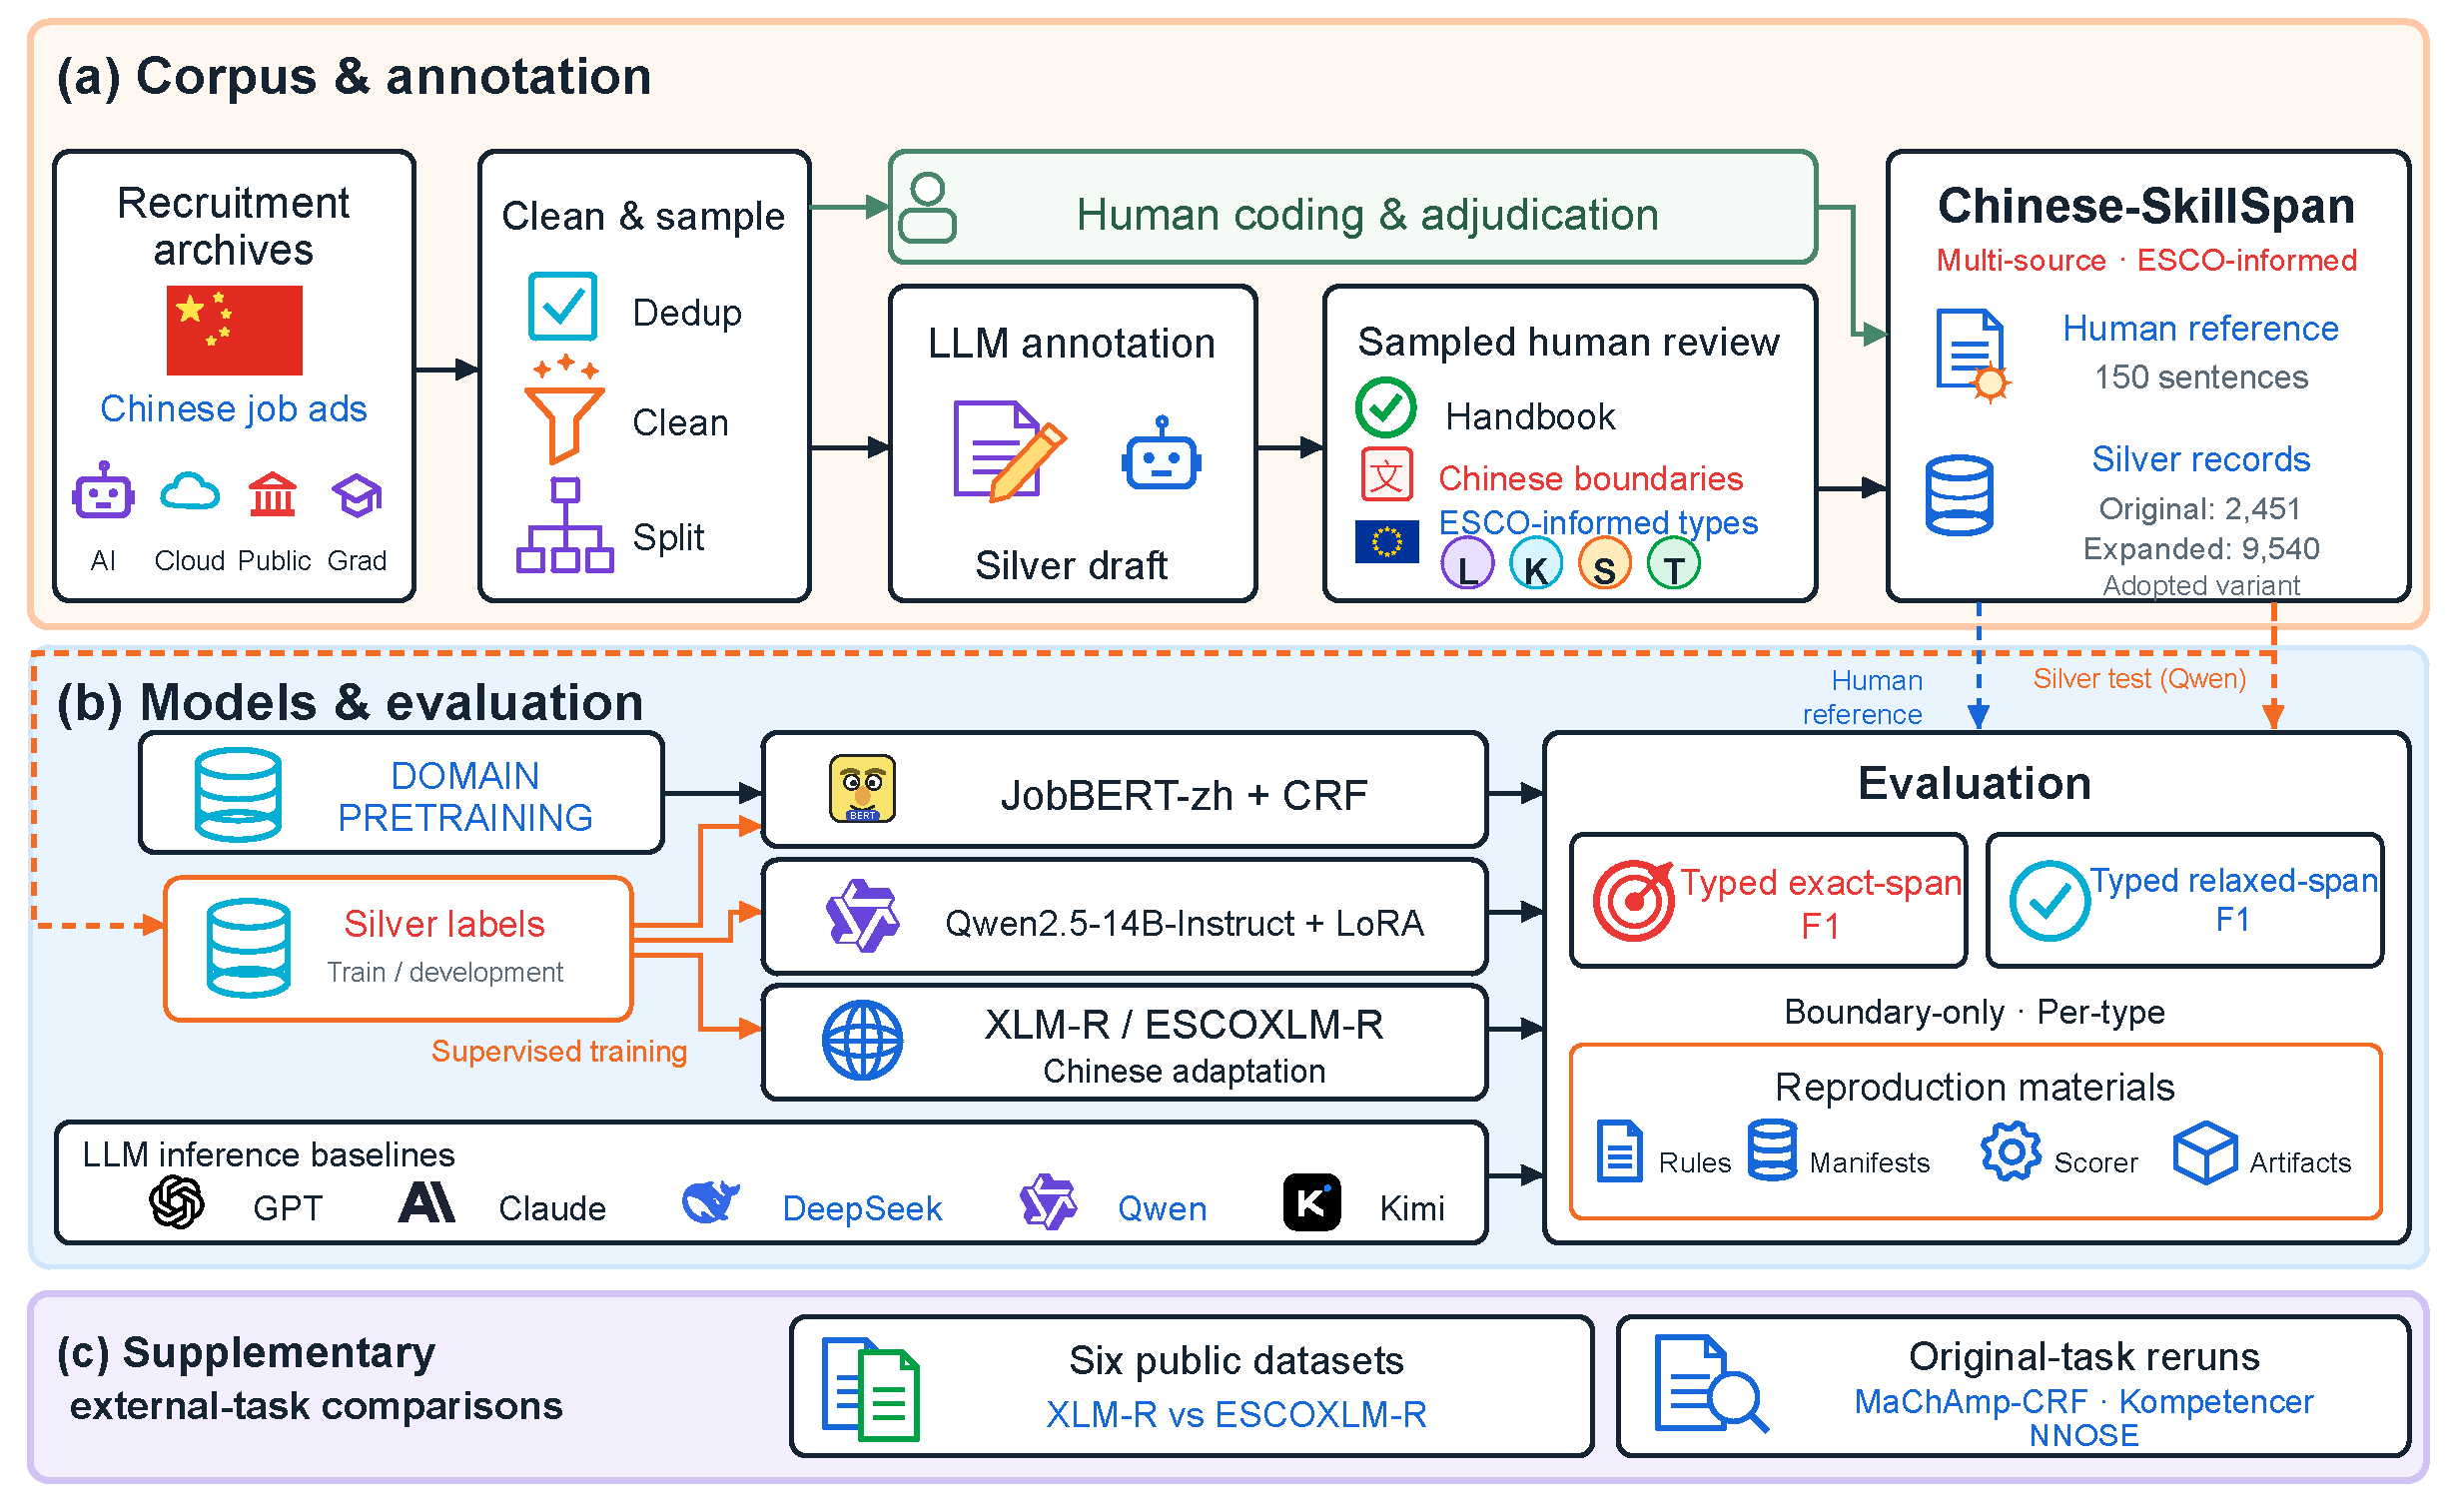
\includegraphics[width=\textwidth]{figures/Figure1_drawio_restored_20261004.pdf}
\caption{Overview of Chinese-SkillSpan: (a) corpus preparation and annotation; (b) model training and evaluation; and (c) supplementary external-task comparisons. Initial layout assisted by OpenAI image generation; final vector drawing prepared with Codex-assisted code (\hyperref[app:d]{Appendix~D}).}
  \label{fig:macro-micro}
\end{figure}

Figure~\ref{fig:macro-micro} summarizes corpus preparation, annotation, and model evaluation. The four categories in Table~\ref{tab:guide-types} draw on ESCO and the knowledge--skill distinction in the European Qualifications Framework~\citep{ESCOv1_2_2024,council2017eqf}.

The definitions and rule examples below illustrate the current handbook, v4.2.14, also used in the blinded agreement study. The human reference retains v4.2.10 labels, whereas the original bulk-generation prompt follows v4.2.12. Current examples do not revise historical annotations; \hyperref[sec:guide-version-history]{Appendix A.4} documents the version boundaries.

\begin{table}[!htbp]
\caption{Operational L/K/S/T definitions and illustrative Chinese spans under handbook v4.2.14.}
\label{tab:guide-types}
\centering\small
\setlength{\tabcolsep}{4pt}
\renewcommand{\arraystretch}{1.12}
\begin{tabularx}{\linewidth}{@{}P{0.19\linewidth}P{0.47\linewidth}L@{}}
\toprule
Label & Operational definition & Chinese examples and English glosses \\
\midrule
L: Language & Natural-language names, proficiency levels, examinations, and certificates. & \zh{英语六级}\par\emph{College English Test Band 6}\par\smallskip\zh{日语N2}\par\emph{Japanese proficiency at N2 level} \\[3pt]
K: Knowledge-related requirements & Facts, principles, theories, and fields of study; educational and non-language qualifications; and explicit industry-background requirements. & \zh{SQL原理}\par\emph{Principles of SQL}\par\smallskip\zh{本科及以上学历}\par\emph{Bachelor's degree or higher} \\[3pt]
S: Occupational skill & Occupational activities and the application of tools or methods. & \zh{使用}[\zh{SQL}]\par\emph{Use [SQL]}\par\smallskip\zh{数据分析}\par\emph{Data analysis} \\[3pt]
T: Transversal competency & General communication, cooperation, cognition, self-management, and dispositions. & \zh{客户汇报}\par\emph{Reporting to clients}\par\smallskip\zh{责任心}\par\emph{Sense of responsibility} \\
\bottomrule
\end{tabularx}
\end{table}


K combines substantive knowledge with recruitment proxies by project convention; qualifications and industry background are not treated as measures of knowledge under ESCO or the EQF. Its scores therefore describe this combined category. The frozen labels do not distinguish these subtypes, so a knowledge-only evaluation would require additional human review.

\begin{figure}[htbp]
\centering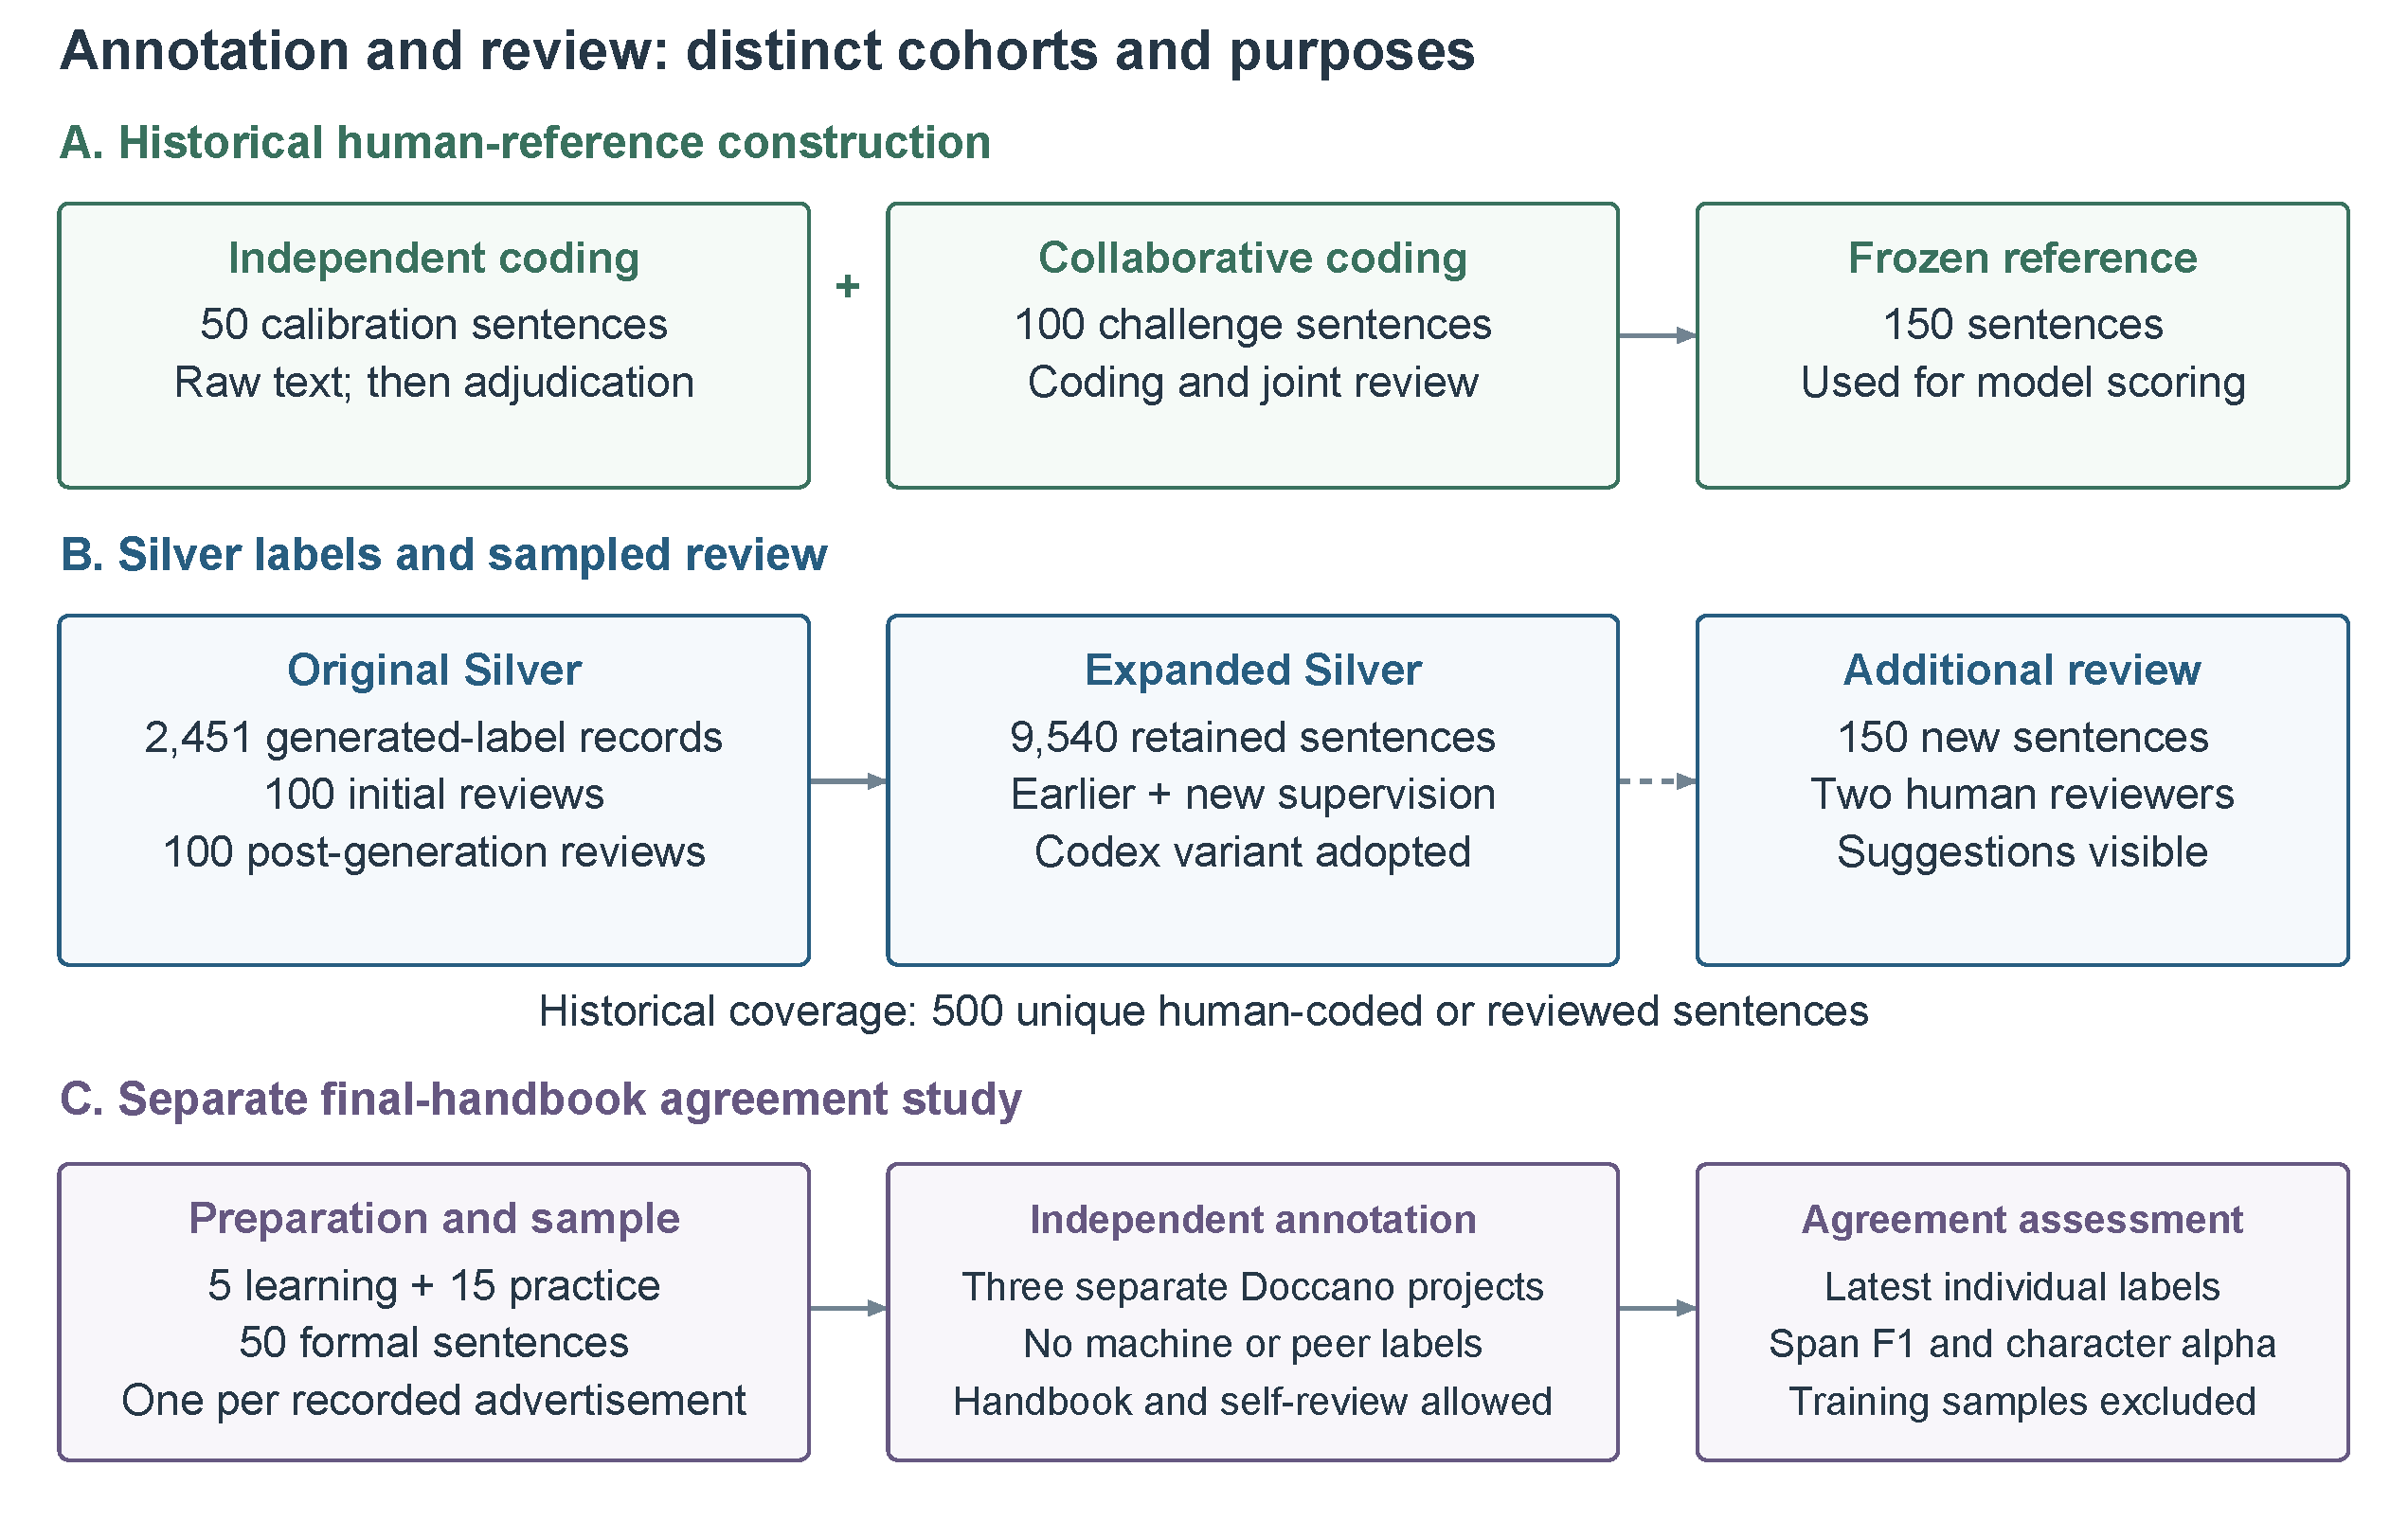
\includegraphics[width=\linewidth]{figures/annotation_paths_major_revision_20261004.pdf}
\caption{Annotation cohorts and their roles. Historical coding and review cover 500 unique sentences. The separate agreement study uses the latest individual annotations after self-review; its five learning and 15 practice sentences are excluded from agreement.}
\label{fig:coding-detail}
\end{figure}


\subsection{Data Sources and Annotation Layers}
\label{sec:challenge-audit}

The source corpus contains 22,840 sentences from four collection batches: AI, Cloud, public-sector, and graduate recruitment. Texts came from commercial collections purchased from MacroData~\citep{macrodataPlatform}, public-institution announcements collected by the research team, and the Recruitment Dataset on Alibaba Cloud Tianchi~\citep{tianchiRecruitment163746}. For the public-institution subset, the team selected government, university, hospital, and public recruitment websites across China, then screened and cleaned the collected texts. The batches can overlap in occupational coverage.

Table~\ref{tab:annotation-lineage} summarizes the principal annotation layers and their uses, following guidance on dataset documentation~\citep{bender2018datastatements,gebru2021datasheets}. The human reference provides evaluation labels, while records selected from the original silver pool provide training and development labels. The adopted expanded silver pool combines earlier supervision with additional cloud, public-sector, and listed-company recruitment texts selected using requirement-related keywords. The model-specific training and development splits are described in \nameref{sec:experiments}.

\begin{table}[!htbp]
\caption{Source corpus and principal annotation layers in Chinese-SkillSpan.}
\label{tab:annotation-lineage}
\centering\small
\setlength{\tabcolsep}{4pt}
\begin{tabularx}{\linewidth}{@{}P{0.20\linewidth}P{0.18\linewidth}P{0.31\linewidth}L@{}}
\toprule
Subset & Size & Annotation content & Role \\
\midrule
Source corpus & 22,840 sentences & Recruitment text from four collection batches & Source material for annotation \\
Human reference & 150 sentences & 663 spans; 8 sentences with no spans (5.3\%) & Model evaluation \\
Original silver pool & 2,451 records & Model-generated annotations with sampled human review & Candidate supervision \\
Adopted expanded silver & 9,540 records & 21,101 spans; 2,492 records with no spans (26.1\%) & Expanded supervision and evaluation against silver targets \\
\bottomrule
\end{tabularx}
\par\smallskip
{\footnotesize\RaggedRight Pool sizes count annotation records, which may repeat a sentence. The layers overlap in source material and should not be summed.\par}
\end{table}

The human reference contains 663 spans: 448 S, 125 K, 88 T, and two L. The 150 sentences have distinct complete texts after Unicode Normalization Form C (NFC). This operation gives equivalent character sequences a consistent representation for comparison. An alternative expanded pool contains 9,646 records and supports a supplementary annotation-channel comparison. \hyperref[app:d]{Appendix D} details both expanded pools' source partitions, composition, and \mbox{selection criteria}.


\subsection{Annotation Guidelines and Adjudication}
\label{sec:annotation-guidelines-r36}

Scope is determined clause by clause. Benefits, application procedures, company promotion, and outcomes alone are excluded; recruitment activities may qualify when they are occupational duties. Thus, \zh{五险一金} (social insurance and housing fund benefits) receives an empty annotation, whereas \zh{能力提升} (capability improvement) without sufficient context remains unresolved. Confirmed absence of an in-scope mention is distinguished from missing context or uncertain interpretation, including in mixed clauses.

Boundary selection prioritizes semantic completeness. Following SkillSpan~\citep{zhang2022skillspan}, annotators retain the shortest complete source span, with no fixed length limit or added words. Generic proficiency triggers usually remain outside the span, but necessary heads and complements remain inside; \zh{会聊天} (can converse) retains its modal as a complete capability expression. Coordinated items are split only when each remains interpretable in context. For example, \zh{熟悉使用Word，Excel，PPT等办公软件} (familiar with office software such as Word, Excel, and PowerPoint) permits separate Word, Excel, and PPT spans. In contrast, \zh{优化曝光与转化率} (optimize exposure and conversion rate) remains one S span because the objects require the shared optimization action.

Experience wording is assessed by distinguishing occupational activities, generic tenure, and industry background. Generic duration alone is excluded; explicit industry-background requirements receive the project-specific K label. For a named activity, annotators remove the experience qualifier only if the remaining words still express the requirement in context. Thus, \zh{机器人竞赛经验} (robotics competition experience) retains its qualifier when the bare event name would change the requirement. Coordinated items must each pass the same test. \hyperref[app:a]{Appendix A} illustrates how internet-company operations receive S while an industry-background requirement receives K.

Type depends on the requirement in context: \zh{使用SQL} (use SQL) supports S for SQL, whereas \zh{了解SQL原理} (understand SQL principles) supports K for \zh{SQL原理} (SQL principles). A predicate can determine type while remaining outside the span; familiarity alone does not determine type. General communication and coordination receive T even in duty clauses, whereas technical operations receive S. Adjudication resolves scope, boundaries, and type separately, without a global label priority~\citep{artstein2008agreement}. Once scope and boundaries are resolved, type-only uncertainty may receive provisional S in the working record, with alternatives logged. All records with unresolved uncertainty are excluded in full from final training targets; provisional S is not an accepted default. Alternative annotations, nested candidates, and unresolved overlaps remain separate from the final flat layer. Figure~\ref{fig:illustrative-annotations} shows frozen human-reference examples; \hyperref[app:a]{Appendix A} retains the complete G1--G15 rules.

\begin{figure}[!htbp]
\centering
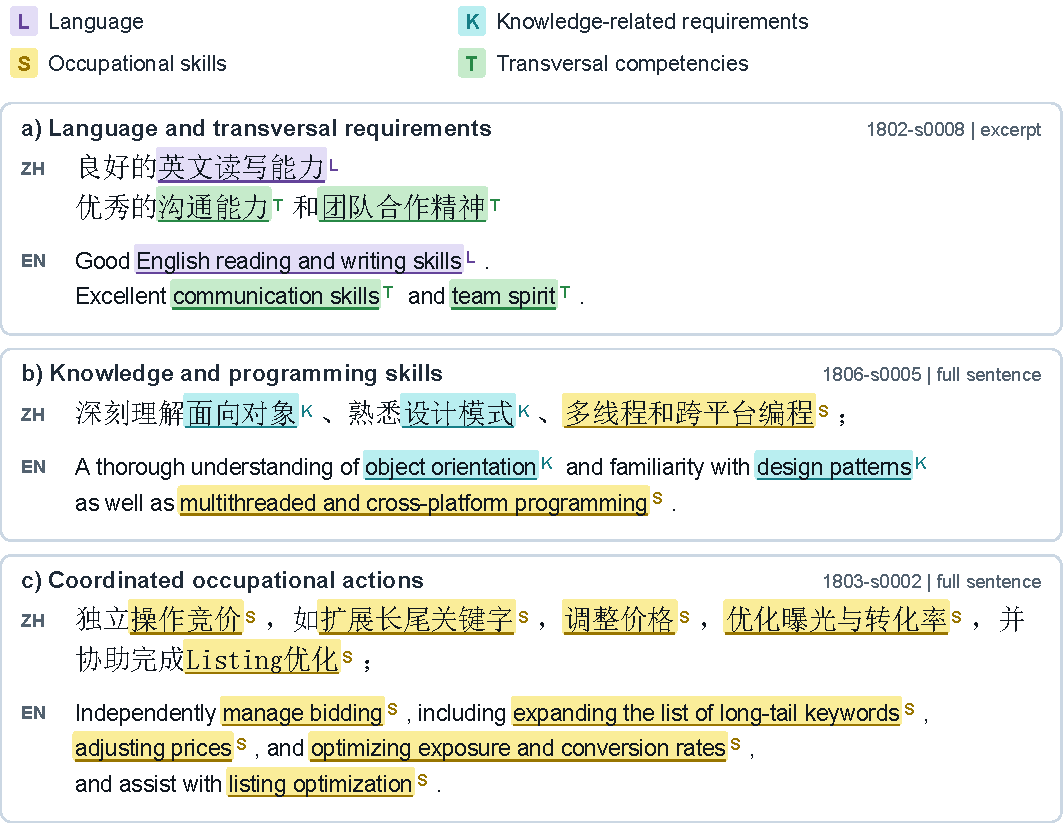
\includegraphics[width=\linewidth]{figures/annotation_examples_main_20261006.pdf}
\caption{Chinese human-reference spans with aligned English translations. Matching colors and labels indicate span correspondences; Chinese highlights reproduce the original reference labels (metadata: v4.2.10).}
\label{fig:illustrative-annotations}
\end{figure}


\subsection{Human Annotation and LLM-Assisted Labeling}
\label{sec:annotation-workflow-r36}

Human annotation, review, and adjudication established the human reference set and informed handbook development. The LLM-labeling route in Figure~\ref{fig:macro-micro} concerns Silver supervision. The adopted annotation route used the official OpenAI Codex interface. In this paper, Codex identifies the interface; Table~\ref{tab:model-identity} lists the recorded model names and their roles. An initial sample review preceded bulk annotation. Automated checks examined span text, offsets, labels, and record coverage, while sampled human review assessed the interpretation of requirements. Each annotation batch used the handbook version available at the time of generation, with later amendments documented separately.

In the adopted expanded-Silver variant, annotations for the designated replacement subset were generated through Codex. Earlier supervision components were retained in both pools, and the alternative variant is reported as a supplementary comparison. Appendices~A~and~D document the handbook versions, record-inclusion decisions, and exclusion of unresolved records.

\FloatBarrier

\subsection{Annotation Quality and Reference Freezing}
\label{sec:annotation-quality}

Agreement must be measured without shared suggestions if it is to assess how consistently annotators apply the handbook. We therefore report the independent blinded study in Table~\ref{tab:quality-main}. Historical coding and assisted-review studies used different samples and rules; their scores cannot be read as a longitudinal improvement in independent reliability (\hyperref[app:b]{Appendix B}).

\paragraph{Blinded coding protocol.}
Three annotators used handbook B.sop\_v4.2.14 after familiarization and training on sets of five and 15 sentences, following the training-and-feedback approach discussed by \citet{klie2024annotationquality}. They then independently coded the same random sample of 50 Silver teacher-pool sentences in separate Doccano projects, blinded to both machine suggestions and one another's labels. Training sentences are excluded from formal agreement. The sample contains one sentence from each of 50 recorded advertisement identifiers; it assesses annotation agreement and is not a new model test set. Source counts and sampling-record limits appear in \hyperref[app:b]{Appendix B}.

We computed agreement from the preserved pre-discussion exports, retaining all 50 sentences and all three coder pairs. Typed exact F1 measures agreement on complete spans without designating a coder as gold~\citep{hripcsak2005agreement}; boundary-only F1 ignores type. Nominal Krippendorff's $\alpha$ uses L/K/S/T/O assignments to all 2,111 source code points. Percentile 95\% intervals use 10,000 source-stratified sentence-bootstrap samples, retaining all three annotations together. These intervals condition on the observed source mixture and coders.

\begin{table}[htbp]
\caption{Independent blinded agreement among three annotators on 50 sentences. Character coefficients are Cohen's $\kappa$ unless marked $\alpha$. Brackets give 95\% bootstrap intervals for typed exact F1. ``Equal'' counts identical sentence-level span sets. Training samples are excluded.}
\label{tab:quality-main}
\centering\small
\begin{tabularx}{\linewidth}{@{}p{0.22\linewidth}rp{0.09\linewidth}p{0.21\linewidth}L@{}}
\toprule
Comparison & $n$ & Character & Typed F1 & Details \\
\midrule
\multicolumn{5}{@{}l}{\textit{Final-handbook independent blinded coding}} \\
A--B & 50 & 0.800 & \makecell[l]{0.657\\{}[0.528, 0.767]} & Boundary F1 0.762; equal 26/50 \\
A--C & 50 & 0.848 & \makecell[l]{0.739\\{}[0.612, 0.850]} & Boundary F1 0.788; equal 33/50 \\
B--C & 50 & 0.803 & \makecell[l]{0.594\\{}[0.459, 0.717]} & Boundary F1 0.721; equal 22/50 \\
Mean / three-rater & 50 & $\alpha$ 0.817 & \makecell[l]{0.663\\{}[0.562, 0.759]} & Mean boundary F1 0.757; all three equal 21/50 \\
\bottomrule
\end{tabularx}
\end{table}

Independent blinded coding leaves substantial span-level disagreement. Mean typed F1 is 0.663, below the planned 0.80 project target, which is not a universal reliability cutoff. Boundary F1 is higher at 0.757 (95\% CI [0.654, 0.846]), indicating additional type disagreement. Character-level $\alpha=0.817$ (95\% CI [0.755, 0.873]) measures a different unit and does not override these span disagreements~\citep{artstein2008agreement}. Of the 21 fully agreed sentences, ten are empty. The two L spans occur in one sentence, limiting category-level conclusions. Frozen labels and diagnostics accompany the \href{https://github.com/AlfredJamesLi/chinese-skillspan-benchmark/tree/main/reproduction/agreement/finalguide_abc_20261002}{reproduction materials}.


\subsection{Ethics and Data Use}
The study analyzed recruitment advertisements and did not recruit job applicants or collect applicant responses. Annotation and review were conducted by members of the research team. Institutional ethics approval was not sought, and no formal exemption is claimed. The authors confirm permission to use the source materials for academic research. Research-use permissions and rights to redistribute third-party recruitment texts are documented separately in the access terms for each component. \hyperref[app:d]{Appendix D} reports the automated privacy-screening results and the human review still required before a privacy-vetted release.

\section{Evaluation Protocol}
\label{sec:experiments}

The evaluation covers prompted extraction, silver-supervised Qwen adaptation, and encoder initialization for Chinese competency extraction, with diagnostics by type, span length, and false positives on sentences without reference spans. The human reference set provides primary evaluation targets; supplementary silver validation and test scores measure agreement with generated annotations.

\subsection{Datasets and Splits}

The original corpus was partitioned by source document into training, development, and test sets with 1,600, 200, and 200 document identifiers, respectively. These partitions share no document identifiers and differ from the later labeled splits used for Silver supervision and human-reference evaluation.

We checked the Silver training and development sets for sentence-level overlap. JobBERT-zh + CRF uses Silver sets of 2,156 training and 169 development records. For Qwen and the encoder comparison, six training records matching three development texts after NFC normalization were removed, leaving 2,150 training and 169 development records. In this split, training and development share no identical or NFC-normalized complete texts, and neither contains a human-reference sentence by identifier or normalized text.

An audit of source-document identifiers found that the 2,150-record Silver training set shared one group with development and 59 groups with the human reference set. The latter contain 143 of the 150 reference sentences. These are different sentences from shared documents, which may contain multiple job postings. Reference sentences are excluded from supervised inputs, but their source documents overlap with training data.

Supplementary expanded-pool Qwen experiments use 8,842/348/350 training/validation/test records from the adopted expanded pool and 8,943/351/352 from the alternative pool. Both combine earlier supervision with additional annotations and differ in annotation channel and included records. Records shared across annotation-channel variants keep their split assignments. Checkpoints are selected by typed exact-span F1 on Silver validation labels. Silver-test scores measure agreement with generated labels in a separate sentence split whose source-document groups overlap with training. Sentence-level checks also excluded human-reference sentences from expanded-model fitting and checkpoint selection. Expanded-model settings and results appear in \hyperref[app:c]{Appendix~C}; duplicate records, normalization checks, and source-group overlaps appear in \hyperref[app:d]{Appendix~D}.

\subsection{Evaluation Metrics}

The primary metric is typed exact-span micro-F1: a match requires identical span boundaries and L/K/S/T type. Typed relaxed-span micro-F1 uses one-to-one greedy matching of same-type spans with intersection-over-union (IoU) of at least 0.5:

\begin{equation}
\mathrm{IoU}(u,v)=\frac{|u\cap v|}{|u\cup v|},
\qquad \mathrm{IoU}(u,v)\geq 0.5.
\label{eq:span-iou}
\end{equation}

Here, $u$ and $v$ are the sets of Unicode-code-point positions in the predicted and reference spans; $\lvert\cdot\rvert$ counts positions. Under either matching rule, true positives (TP) are matched prediction--reference pairs, false positives (FP) are unmatched predictions, and false negatives (FN) are unmatched reference spans. Counts are summed across sentences before computing the micro-averaged metrics:

\begin{equation}
P_{\mathrm{micro}}=\frac{\mathrm{TP}}{\mathrm{TP}+\mathrm{FP}},
\quad R_{\mathrm{micro}}=\frac{\mathrm{TP}}{\mathrm{TP}+\mathrm{FN}},
\quad F_{1,\mathrm{micro}}=\frac{2\mathrm{TP}}{2\mathrm{TP}+\mathrm{FP}+\mathrm{FN}}.
\label{eq:micro-prf}
\end{equation}

When a denominator is zero, the corresponding precision, recall, or F1 is set to zero. All 150 sentences in the human reference set are scored. Expanded Qwen runs also report silver validation and test scores. Accepted spans from partially rejected responses remain in scoring; malformed responses and responses with no accepted spans yield empty predictions. A sentence with no predicted or reference spans contributes no TP, FP, or FN counts. \hyperref[app:c]{Appendix C} gives parser rules and matching order and links the scoring implementation.

Boundary-only exact-span micro-F1 ignores type and matches span boundaries. Per-type scores are computed over all reference sentences, including those without any reference span of the evaluated type. Macro-F1 is the arithmetic mean of F1 over the specified categories.

\begin{samepage}
For experiments repeated across three training seeds, we report the mean and sample standard deviation, where $f_i$ is the score from run $i$:
\par\nopagebreak[4]

\begin{equation}
\bar f=\frac{1}{n}\sum_{i=1}^{n}f_i,
\qquad s_f=\sqrt{\frac{1}{n-1}\sum_{i=1}^{n}(f_i-\bar f)^2},
\qquad n=3.
\label{eq:seed-summary}
\end{equation}
\par\end{samepage}

Inference-only configurations and expanded-pool experiments are single runs unless otherwise stated. For paired model comparisons, 95\% percentile intervals are obtained from 10,000 bootstrap resamples of the 61 source-document groups in the human reference set. Complete groups are sampled with replacement, using the same draw for all compared models. These intervals describe uncertainty from resampling the reference set for the evaluated runs; training-seed standard deviations describe variation across training runs. \hyperref[app:c]{Appendix C} provides the full resampling procedure.

\subsection{Models and Baselines}

JobBERT-zh is a sequence-labeling baseline with a Chinese recruitment-domain-pretrained encoder and a CRF head. We compare Qwen2.5-14B-Instruct (Qwen)~\citep{qwen2025report} with and without a project-trained LoRA adapter~\citep{hu2022lora} for generative extraction.

The prompted comparison uses shared annotation instructions across GPT-5.6 Terra, Claude Sonnet 4.5, DeepSeek-V4-Pro (DeepSeek), Kimi K2.6 (Kimi), and Qwen without a project adapter. DeepSeek is evaluated with thinking enabled and disabled, giving six configurations. GPT-5.6 Terra and Claude Sonnet 4.5 were accessed through an API gateway. Table~\ref{tab:model-identity} lists model identifiers, access routes, and key settings.

The adopted Silver annotation route used the Codex configuration in Table~\ref{tab:model-identity}, and the GPT baseline used a separate API configuration. Shared guidelines and assisted review can nevertheless align annotation choices across these configurations, limiting the independence of their errors.

\begin{table}[!htbp]
\centering\small
\caption{Recorded model identifiers and access routes by study role.}
\label{tab:model-identity}
\begin{tabularx}{\linewidth}{@{}P{.19\linewidth}P{.32\linewidth}L@{}}
\toprule
Configuration / role & Recorded identifier & Access and key settings \\
\midrule
\multicolumn{3}{@{}l}{\textit{Evaluation configurations}} \\
GPT (API) & Request: \texttt{gpt-5.4}; returned: \texttt{gpt-5.6-terra} & API gateway; temperature 0; cap 2,048 tokens. \\
Claude (API) & \texttt{claude-sonnet-4-5-20250929} & API gateway; temperature 0; cap 2,048 tokens. \\
DeepSeek (API) & \texttt{deepseek-v4-pro} & Official \href{https://api.deepseek.com}{DeepSeek API}; non-thinking: temperature 0, cap 2,048; thinking: cap 8,192, temperature unspecified. \\
Kimi (API) & \texttt{kimi-k2.6} & Official \href{https://api.moonshot.cn}{Moonshot API}; non-thinking; temperature 0.6; cap 2,048. \\
Qwen (unadapted / LoRA) & Qwen2.5-14B-Instruct & Local weights; deterministic decoding; cap 2,048. \\
JobBERT-zh + CRF & Released initialization and Silver-trained continuation & Local encoder and inherited CRF. \\
\midrule
\multicolumn{3}{@{}l}{\textit{Annotation and assisted review}} \\
Original silver annotation & \texttt{gpt-6-astra} & Official OpenAI Codex; adopted original silver labels. \\
Expansion comparison & Codex selection / API-returned \texttt{gpt-6-astra} & Codex / API gateway; 2,500-candidate replacement batch only; earlier components shared. \\
Additional review & \texttt{gpt-6-astra}; Grok 4.6-high & Codex / Cursor; suggestions visible to reviewers. \\
Annotation support & Qwen; DeepSeek; Kimi & Machine-generated annotation suggestions. \\
\bottomrule
\end{tabularx}
\par\smallskip\footnotesize\RaggedRight
Caps are output-token limits. Codex and Cursor denote interfaces. GPT and Claude gateway identities were not independently verified against vendor APIs. \hyperref[app:c]{Appendix C} gives available run settings; \hyperref[app:d]{Appendix D} records checkpoint provenance and historical implementation gaps.
\end{table}


\subsection{Implementation Details}

\paragraph{Supervision and model selection.} JobBERT conditions start from the same released encoder and CRF. Earlier supervision (B1 in the experiment files) uses the historical extraction labels; revised supervision (B2) combines updated guidance, LLM annotation, and adjudication. The conditions share training and development texts, with label changes in 1,440 training records and 107 development records. Development typed exact F1 selects checkpoints, so this comparison changes training supervision and selection targets together.

Qwen starts from its pretrained Instruct weights and fits a fresh LoRA adapter for each of seeds 42, 43, and 44 on the revised 2,150/169 split. Training uses a fixed system instruction, user template, and five schematic examples. Targets contain the literal span text, occurrence index, and type. Loss applies to the assistant JSON and closing turn token. Training uses BF16, and development exact F1 selects the adapter. Table~\ref{tab:training-settings} gives the remaining settings. Historical JobBERT implementation gaps are documented in \hyperref[app:d]{Appendix D}.

\begin{table}[htbp]
\centering
\caption{Original JobBERT and Qwen training settings. Both select checkpoints by development typed exact F1; reproduction notes retain implementation and selection records.}
\label{tab:training-settings}
\small
\begin{tabularx}{\linewidth}{@{}P{0.27\linewidth}P{0.27\linewidth}L@{}}
\toprule
Setting & JobBERT-zh B1/B2 & Qwen LoRA \\
\midrule
Learning rate & $2\times10^{-5}$ & $10^{-4}$ \\
Batch size & 16 & 1; 16-step gradient accumulation \\
Maximum input length & 256 tokens & 8,192 tokens \\
Training limit & 6 epochs; patience 2 & 6 epochs; patience 2 \\
\bottomrule
\end{tabularx}
\par\smallskip\RaggedRight\footnotesize Qwen uses LoRA with rank 16, scaling 32, and dropout 0.05, applied to the attention q/k/v/o projections.
\end{table}

\paragraph{Inference.} Each request contains one sentence's identifier and text, together with the shared instruction and five fixed examples. A parser converts occurrence-based output into character spans. Qwen baseline and adapter inference use the same base checkpoint, prompts, parser, BF16 precision, deterministic decoding, and 2,048-token output cap. DeepSeek uses caps of 2,048 tokens without thinking and 8,192 with thinking. \hyperref[app:c]{\mbox{Appendix~C}} lists service settings and output checks.


\phantomsection
\label{sec:external-benchmark-plan}

To assess taxonomy-informed initialization, we compare \href{https://huggingface.co/FacebookAI/xlm-roberta-large}{XLM-R-large}~\citep{conneau2020xlmr} and \href{https://huggingface.co/jjzha/esco-xlm-roberta-large}{ESCOXLM-R}~\citep{zhang2023escoxlmr} with newly initialized nine-label BIO heads. The pair uses the same silver split, training settings, and checkpoint-selection criterion. Different prediction heads and training budgets make comparisons with JobBERT and Qwen descriptive.


\section{Results}
\label{sec:results-r12}

\subsection{Prompted Inference on the Human Reference Set}

GPT-5.6 Terra achieved the highest observed typed exact-span micro-F1 among the six configurations, scoring 0.667 compared with 0.647 for DeepSeek with thinking disabled (Table~\ref{tab:gold150-shared-r7}). Their paired difference was 0.020, with a 95\% source-group bootstrap interval of $[-0.027, 0.061]$ (Table~\ref{tab:core-paired}). The interval includes zero, so the observed lead is not clearly resolved by this comparison.

These end-to-end scores apply to the prompts, output budgets, and parsing rules specified in the evaluation protocol. Qwen without an adapter had the lowest recall at 0.281.

% [Stage2] Core metrics and cohort appendix share stage2_result_values.tex.
\begin{table}[H]
\caption{Shared-guideline inference configurations on the human reference ($n=150$). P/R are typed exact precision/recall. Each configuration is a single run. Inference budgets are configuration-specific. Qwen uses no project adapter.}
\label{tab:gold150-shared-r7}
\centering\small
\newcommand{\SharedResultRow}[7]{#1 & #2 & #3 & #4 & #5 \\}
\begin{tabularx}{\linewidth}{@{}Lrrrr@{}}
\toprule
Recorded configuration & P & R & Exact F1 & Relaxed F1 \\
\midrule
\SharedResultRows
\bottomrule
\end{tabularx}
\par\smallskip\footnotesize\RaggedRight
Both DeepSeek rows use the same model. Non-thinking and thinking denote inference modes, with output caps of 2,048 and 8,192 tokens respectively. Table~\ref{tab:model-identity} lists the recorded identifiers, access routes, and settings. Cohort scores and detailed output-status counts accompany the reproduction materials.
\end{table}

\begin{table}[!htbp]
\centering\small
\caption{Paired typed exact-F1 differences on the human reference, with 95\% intervals from resampling the 61 source-ID groups.}
\label{tab:core-paired}
\begin{tabularx}{\linewidth}{@{}Lrr@{}}
\toprule Comparison & Difference & 95\% interval \\\midrule
GPT (API) minus DeepSeek non-thinking & ${+0.020}$ & $[-0.027, 0.061]$ \\
Qwen LoRA 42 minus no adapter & ${+0.138}$ & $[0.069, 0.200]$ \\
Qwen LoRA 43 minus no adapter & ${+0.202}$ & $[0.133, 0.269]$ \\
Qwen LoRA 44 minus no adapter & ${+0.197}$ & $[0.123, 0.268]$ \\
Qwen LoRA seed mean minus no adapter & ${+0.179}$ & $[0.111, 0.242]$ \\
ESCOXLM-R minus XLM-R-large & ${+0.016}$ & $[-0.005, 0.035]$ \\
\bottomrule
\end{tabularx}
\par\smallskip\RaggedRight\footnotesize Each bootstrap draw resamples complete source-ID groups with replacement and uses the same draw for all models. Intervals condition on the recorded runs and reference; they are pointwise and do not establish independence from guideline development.
\end{table}

\subsection{Silver-Supervised Adaptation}
\label{sec:silver-results}

Silver supervision improved Qwen's typed exact-span micro-F1 under the fixed inference protocol. The adapted mean was $0.540\pm0.035$, compared with 0.361 without an adapter (Figure~\ref{fig:model-comparison}b; Table~\ref{tab:gold150-main}, panel A). The mean gain over the three training seeds was 0.179, with a paired 95\% bootstrap interval of $[0.111, 0.242]$; the intervals for all three individual seeds also lay above zero (Table~\ref{tab:core-paired}). Mean scores also increased under relaxed and boundary-only matching, showing gains across the three matching criteria.

The adapters produced fewer responses with rejected span candidates than the unadapted model. These end-to-end scores reflect both span extraction and output validity. The reproduction materials include \href{https://github.com/AlfredJamesLi/chinese-skillspan-benchmark/blob/1d1c24e20ee049fc768034b5baf58fa882e08e2c/reproduction/process_archive_20260924/secondary_review/tables/qwen_per_seed.csv}{per-seed Qwen scores} and parser outcomes.

The silver-trained JobBERT-zh + CRF baseline achieved mean typed exact-span micro-F1 of $0.554\pm0.005$ (Figure~\ref{fig:model-comparison}b; Table~\ref{tab:gold150-main}, panel B). Its mean exceeded Qwen + LoRA (0.540), while both remained below prompted GPT-5.6 Terra (0.667). These rankings describe the evaluated configurations, whose training and inference protocols differ across model families.


\subsection{Supplementary Analyses}

Each Qwen adapter increased exact-match recall in all three reference-span length bins: $\leq4$, 5--8, and $\geq9$ Unicode code points (Figure~\ref{fig:qwen-diagnostics}). These bins contain 346, 243, and 74 reference spans, respectively.

On the eight sentences with no reference spans, the number of false-positive spans decreased from 19 without an adapter to 6, 4, and 0 for seeds 42, 43, and 44. The unadapted run produced false positives in two sentences; the adapted runs affected two, one, and zero sentences, respectively. For seed 42, the reduction occurred within the same two affected sentences.

\begin{figure}[!htbp]
\centering
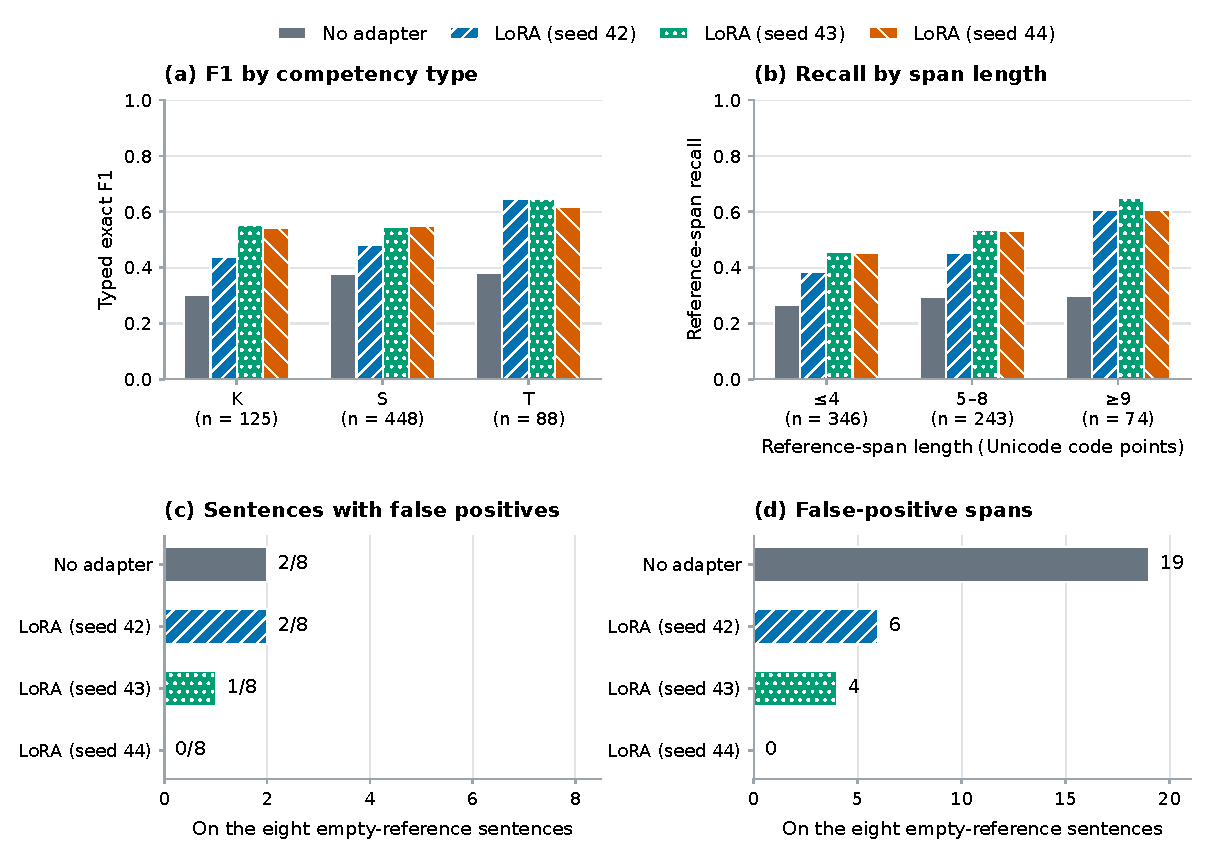
\includegraphics[width=\linewidth]{figures/qwen_diagnostics_chart_0913.pdf}
\caption{Qwen diagnostics on the human reference set: (a) typed exact-span F1 by type; (b) recall by reference-span length ($n$: reference spans); (c--d) false positives on eight sentences with no reference spans, counted by sentence and span.}
\label{fig:qwen-diagnostics}
\end{figure}


\subsection{Encoder and Competency-Type Comparisons}
\label{sec:external-benchmark-results}

XLM-R-large and ESCOXLM-R achieved mean typed exact-span micro-F1 scores of 0.522 and 0.538, respectively (Table~\ref{tab:external-chinese}, panel A). Scores were recomputed from all six archived prediction files against the same human reference set. The mean difference was 0.016, with a paired 95\% interval of $[-0.005, 0.035]$ (Table~\ref{tab:core-paired}). The interval includes zero and does not establish an advantage for ESCO initialization under this protocol.

Four-type macro-F1 was 0.607 for XLM-R-large and 0.622 for ESCOXLM-R. Averaging over K/S/T gave 0.542 and 0.562, respectively. These sensitivity summaries exclude the sparsely represented L category from the macro average without changing the four-type prediction task.

Qwen adaptation improved all three K/S/T categories (Table~\ref{tab:external-chinese}, panel B; Figure~\ref{fig:qwen-diagnostics}). The largest observed increase among these categories was for T, from 0.380 to 0.638. Mean S and K scores increased by 0.148 and 0.210, respectively. Among the three Silver-trained configurations in Table~\ref{tab:external-chinese}, panel B, Qwen had the highest observed mean scores for S and T, while ESCOXLM-R had the highest K score. These rankings are descriptive because prediction heads, training budgets, and inference procedures differ across architectures.

\begin{table}[!htbp]
\centering\small
\caption{Supervised adaptation of multilingual encoders on Gold150 (0--1), mean $\pm$ sample SD across three seeds.}
\label{tab:external-chinese}
\begin{tabularx}{\linewidth}{@{}Lrrrr@{}}
\toprule
Encoder & Typed exact & Typed relaxed & Boundary & Macro-F1 \\
\midrule
XLM-R-large & $0.522\pm0.022$ & $0.650\pm0.021$ & $0.571\pm0.022$ & $0.607\pm0.016$ \\
ESCOXLM-R & $0.538\pm0.021$ & $0.662\pm0.022$ & $0.582\pm0.024$ & $0.622\pm0.010$ \\
\bottomrule
\end{tabularx}
\par\smallskip\RaggedRight\footnotesize B2 training/development: 2,150/169 records. Fresh linear LSKT head; official \texttt{cnss-lskt-1.2.0} scorer; 150 human-reference records. Boundary is exact span matching with types collapsed; macro-F1 averages L/K/S/T. Gold150 is not a new blind test and contains only two L spans. All three seeds (42/43/44) are included; per-seed scores and selected epochs are retained in the model audit archive.
\end{table}

\begin{table}[!htbp]
\centering\small
\caption{Common-protocol typed exact token-span micro-F1 (0--1), mean $\pm$ sample SD across three seeds.}
\label{tab:external-common}
\begin{tabularx}{\linewidth}{@{}L P{.14\linewidth}P{.25\linewidth}rr@{}}
\toprule
Dataset & Stream & Train/dev/test & XLM-R-large & ESCOXLM-R \\
\midrule
SkillSpan & Skill & 4,800/3,174/3,569 & $0.567\pm0.012$ & $0.577\pm0.006$ \\
SkillSpan & Knowledge & 4,800/3,174/3,569 & $0.698\pm0.021$ & $0.672\pm0.052$ \\
Kompetencer & Skill & 778/346/262 & $0.545\pm0.028$ & $0.527\pm0.004$ \\
Kompetencer & Knowledge & 778/346/262 & $0.618\pm0.035$ & $0.593\pm0.044$ \\
Gnehm ICT & ICT & 19,889/2,332/2,557 & $0.891\pm0.005$ & $0.867\pm0.032$ \\
Green & Native types & 8,669/964/335 & $0.493\pm0.009$ & $0.492\pm0.007$ \\
Sayfullina & Skill & 3,705/1,855/1,851 & $0.920\pm0.004$ & $0.925\pm0.005$ \\
FIJO & Native types & 399/50/50 & $0.343\pm0.019$ & $0.339\pm0.007$ \\
\bottomrule
\end{tabularx}
\par\smallskip\RaggedRight\footnotesize Both encoders use fresh linear BIO heads, 20 epochs, and development-set checkpoint selection. SkillSpan and Kompetencer have separate skill and knowledge streams; Green and FIJO retain their entity types. German data use the public ICT release. The shared protocol differs from the original CRF and NNOSE methods.
\end{table}



\subsection{Boundary and Type Disagreements in Human Annotation}

The blinded annotation study found disagreement in both span boundaries and types. Mean boundary-only exact-span F1 was 0.850, compared with 0.818 when matching also required identical types (Table~\ref{tab:quality-main}). The decrease when type matching is required shows that type assignment contributes to disagreement beyond span boundaries.

The agreement study and model evaluation use different texts, label versions, and annotation procedures. Direct comparison of human and model agreement would require evaluating both on a common independently annotated sample.

\subsection{Scoring Criteria and Evaluation Targets}

For the same unadapted Qwen predictions, relaxing the matching criterion raises F1 from 0.361 to 0.470 (Table~\ref{tab:gold150-shared-r7}). Under typed exact matching, the 181 false positives comprise 27 same-boundary/different-type pairs, 89 same-type/overlapping-boundary pairs, and 65 other unmatched predictions. This grouping compares predicted boundaries and types with the reference annotations. A relaxed match still requires the same type and an IoU of at least 0.5.

Two unadapted Qwen outputs illustrate these distinctions. For \texttt{1801-s0004}, the prediction is the S span \zh{参与公司无人机飞控系统技术项目开发策划} (participate in planning a technical development project for the company's UAV flight-control system), whereas an overlapping reference S span is \zh{技术项目开发策划} (technical project development planning). Their overlap is below the relaxed threshold, so this pair matches under neither criterion. For \texttt{1802-s0005}, both layers select \zh{方法} (method), but the prediction is S and the reference is K. This pair has identical boundaries but fails both typed matching rules. Appendix~C gives the complete source sentences and offsets for these prediction--reference comparisons.

The exploratory expanded-pool Qwen runs produced different rankings across evaluation targets. With seed 42, the adopted expanded pool yielded F1 of 0.809 on its Silver test set and 0.585 on the shared human reference, whereas the alternative yielded 0.759 and 0.597, respectively (Table~\ref{tab:expanded-silver-main}). The adopted pool had the higher Silver-test score, and the alternative had the higher human-reference score. The pool-specific Silver tests differ in both texts and labels. The \hyperref[sec:annotation-quality]{annotation-quality analysis} provides the common-sentence comparison against blinded human annotations. Table~\ref{tab:source-stages} gives the constituent batches and final counts.

Exploratory expanded JobBERT results in Appendix~C show lower human-reference scores under jointly changed supervision, source composition, and model selection.

\section{Limitations and Responsible Use}
\label{sec:limitations}

\textbf{Reference design and label scope.} Gold150 is a disagreement-selected reference used in handbook development. The separate 50-sentence agreement study tests use of the final handbook; it does not supply a new held-out model test. Human annotation agreement and model scores use different samples and targets. K includes qualification and industry-background proxies, and L has only two reference spans. Independent annotation of new, advertisement-isolated texts and human review of K subtypes remain necessary to establish broader validity.

\textbf{Historical supervision and access.} The reference, original supervision, and agreement study use different handbook versions. Their labels remain frozen, so final-handbook consistency does not establish compatibility of all historical targets. The original corpus has disjoint source-document partitions, and later B2 checks exclude reference sentences from supervision. The later experimental splits nevertheless share source-document groups, which limits claims about new-document generalization. Incomplete pretraining records leave additional exposure uncertain. Public labels and predictions support inspection and rescoring, while complete expanded-pool inputs are not publicly available for retraining. Reuse must respect the component-specific source permissions.

\textbf{Experimental scope.} The Qwen comparison measures end-to-end gains from adaptation, including improved output validity. It does not isolate a semantic-extraction effect. Prompted configurations differ in inference budgets and access routes, expanded-pool studies use single seeds, and three-seed SD is imprecisely estimated. Source-group bootstrap intervals address dependence among recorded reference prefixes but remain conditional on the selected examples and trained models. Eight empty-reference sentences support descriptive error counts only.

\section{Conclusion}
\label{sec:conclusion}

Chinese-SkillSpan provides a benchmark for delimiting and typing competency mentions in Chinese job advertisements. Its contributions are an original-text resource with distinct human and Silver labels, an ESCO-informed operational handbook for Chinese boundaries and contextual types, and annotation-quality evidence that separates independent agreement from assisted review. Fixed character offsets, released predictions, and a shared scorer make model errors inspectable.

Three independent annotators achieved mean typed exact agreement of 0.818 after individual self-review under the final handbook. Qwen adaptation improved end-to-end extraction against its own base checkpoint, while the prompted GPT configuration remained strongest by point score. The Chinese encoder comparison did not establish an ESCO initialization advantage. Together, these experiments demonstrate use of the resource for diagnostic comparison and identify the additional annotation and independent testing needed for broader deployment.


\section{Acknowledgements}
We thank AML Lab for providing GPU resources and access to OpenAI Codex. Codex assisted with manuscript editing, typesetting, and code and figure preparation; Anthropic Claude supported language editing, and xAI Grok 4.6 supported code checking. OpenAI's image-generation tool informed the initial layout of Figure~\ref{fig:macro-micro}. Some preparation-tool versions were not retained. The authors reviewed AI-assisted material and take full responsibility for the manuscript.

% [R4-LAYOUT] Keep each repository URL intact without forcing an extra page.
\section{Data Availability}
\begin{sloppypar}
\RaggedRight % [R4-LAYOUT] Avoid stretched word spacing around intact URLs.
\setlength{\parindent}{1em}
% Resource locations, reproduction scope and reuse terms; detailed inventory in Appendix D.
The \href{https://doi.org/10.5281/zenodo.22698504}{dataset archive, v0.1.3 (DOI: 10.5281/zenodo.22698504)}, contains the corpus, handbook, 150-sentence human reference, and 2,150/169 silver training/development records used by Qwen and the encoder comparison. This version-specific DOI identifies the dataset used here; the archive series has concept DOI \href{https://doi.org/10.5281/zenodo.22288337}{10.5281/zenodo.22288337}. Later \href{https://github.com/AlfredJamesLi/chinese-skillspan-benchmark/blob/main/reproduction/evidence_review_20260925/annotation_layers/README.md}{historical annotation and assisted-review materials} and the \href{https://github.com/AlfredJamesLi/chinese-skillspan-benchmark/tree/main/reproduction/agreement/finalguide_abc_20261003}{blinded agreement study} are released separately, with pseudonymized annotator identifiers, source texts, offsets, and individual annotation layers.

The \href{https://doi.org/10.5281/zenodo.22851581}{Qwen archive (DOI: 10.5281/zenodo.22851581)} provides three original-silver LoRA adapters, selected expanded-silver checkpoints, predictions, configurations, and scoring tools. For the 9,540-record adopted and 9,646-record alternative expanded pools, split identifiers and selected outputs are public; complete texts and labels are available through the corresponding author for confidential peer review. Six Chinese-supervised XLM-R/ESCOXLM-R checkpoints are linked in the \href{https://github.com/AlfredJamesLi/chinese-skillspan-benchmark/blob/0c73207c0f9b00fa87f385b78bcb7342bd00bfcb/results_snapshots/table11_evidence_20260924/HF_RELEASE.md}{model index}, with code, configurations, and predictions in the \href{https://doi.org/10.5281/zenodo.22942441}{evaluation archive (DOI: 10.5281/zenodo.22942441)}. The \href{https://github.com/AlfredJamesLi/chinese-skillspan-benchmark/blob/main/reproduction/evidence_review_20260925/README.md}{reproduction documentation} separately describes local score recalculation from saved predictions and reported results of model reruns on a server.

The \href{https://huggingface.co/AlfredJames/jobbert-zh}{JobBERT-zh model used for initialization} includes the domain-adapted encoder and existing CRF; the \href{https://huggingface.co/AlfredJames/jobbert-zh-v6a}{silver-trained release} provides silver-trained checkpoints (default: seed 42). The \href{https://github.com/AlfredJamesLi/chinese-skillspan-benchmark}{project repository} and \href{https://github.com/AlfredJamesLi/chinese-skillspan-benchmark/blob/main/REPRODUCIBILITY.md}{reproduction guide} provide code, procedures, and records, including \href{https://github.com/AlfredJamesLi/chinese-skillspan-benchmark/tree/main/reproduction/major_revision_20261004/external_experiments}{supplementary external-task experiments}. Table~\ref{tab:component-access} summarizes access and reproduction scope.

Reuse follows component-specific terms: Apache-2.0 for explicitly covered software and documentation; academic research and peer review with attribution for author-controlled annotations and research materials; source permissions for third-party recruitment texts; and accompanying notices and base-model licences for checkpoints and adapters. The \href{https://github.com/AlfredJamesLi/chinese-skillspan-benchmark/blob/main/DATA_AVAILABILITY.md}{data-access guide} and \hyperref[app:d]{Appendix D} provide the terms and limitations.
\end{sloppypar}

% [R16] Four reader-facing appendices replace chronological/provenance-heavy routing.
% Original inputs remain in the project and the R15 git snapshot; no assets deleted.
% [R16-ROUTE] Author-approved four-part appendix. No original assets deleted.
% Before-image: 7Appendix.tex and former direct inputs remain unchanged.
\FloatBarrier
\appendix
\captionsetup[table]{skip=3pt}
\setlength{\textfloatsep}{8pt}
\setlength{\floatsep}{8pt}
\setlength{\intextsep}{8pt}
% [R17] Editable, example-led visual guide; R16 source remains preserved.
% [R18] Restore rule/decision/highlighted-example tables; retain R17 source.
% [R19] Source-attributed presentation derivative of the bilingual V4.2.14 handbooks.
% Presentation layer: Chinese examples, span boundaries, labels, and execution versions remain unchanged.
% G1--G15 are display identifiers, not new normative rule IDs or a relabelled V4.2.9 image.
% Crosswalk and source hashes: handbooks/ALIGNMENT_R18.md. No annotations are changed.
\definecolor{guideL}{HTML}{DED9F7}
\definecolor{guideK}{HTML}{C6ECEE}
\definecolor{guideS}{HTML}{FFF0B0}
\definecolor{guideT}{HTML}{CDEACF}
\newcommand{\gspan}[2]{{\setlength{\fboxsep}{1.4pt}\colorbox{guide#1}{\strut [#2]\,\textsf{[#1]}}}}
\newcommand{\gcontext}[1]{\textcolor{black!75}{#1}}
\newcommand{\gsource}[1]{\,\textsuperscript{\textsf{[#1]}}}
\newcommand{\ggloss}[1]{\par\emph{#1}}

\section{Appendix A. Coding Guide and Examples}
\phantomsection
\label{app:a}
\label{sec:handbook-current}
This appendix summarizes the v4.2.14 rule series with bilingual examples. Figure~\ref{fig:illustrative-annotations} shows the preserved human-reference annotations. The full \href{https://github.com/AlfredJamesLi/chinese-skillspan-benchmark/blob/main/notes/handbooks/reader_20261007/README.md}{Chinese and English handbooks, dated 7 October 2026}, provide further examples and identify cases awaiting review. Section~A.4 distinguishes these reading materials from the versions associated with the reported studies.

\subsection{A.1 Label definitions and notation}
Table~\ref{tab:guide-types} defines the four labels with examples. Square brackets mark selected source substrings, followed by their type codes. Brackets, colours, and type codes are display aids rather than source characters; brackets keep boundaries identifiable in grayscale. The examples illustrate annotation decisions and are not an additional evaluation sample.

\noindent\textit{Source key.} E: ESCO's \href{https://esco.ec.europa.eu/en/about-esco/escopedia/escopedia/skills-pillar}{skills hierarchy} and \href{https://esco.ec.europa.eu/en/about-esco/escopedia/escopedia/transversal-knowledge-skills-and-competences}{transversal concepts} \citep{ESCOv1_2_2024}; Q: EQF definitions \citep{council2017eqf}; Z: related annotation guidance in SkillSpan, Appendix B \citep{zhang2022skillspan}; I: unitization and categorization in agreement analysis \citep{artstein2008agreement}; P: our V4.2.14 operational decision. Combined marks indicate adaptation, not verbatim rules; Chinese examples and exact boundaries are project illustrations.

\Needspace{8\baselineskip}
\subsection{A.2 General annotation decisions}
G1--G15 are quick-reference identifiers. Their source sections and amendment IDs (R08--R23) are mapped in the release; they do not replace the handbook's rule numbering.

\begingroup
\small\setlength{\tabcolsep}{4pt}\renewcommand{\arraystretch}{1.13}
\begin{longtable}{@{}P{0.07\linewidth}P{0.49\linewidth}P{\dimexpr0.44\linewidth-16pt\relax}@{}}
\caption{Annotation principles for competency mentions and span boundaries.}\label{tab:guide-boundaries}\\
\toprule\textbf{Rule} & \textbf{Annotation principle} & \textbf{Example and English gloss}\\\midrule
\endfirsthead
\multicolumn{3}{@{}l}{\textit{Table \thetable\ (continued)}}\\
\toprule\textbf{Rule} & \textbf{Annotation principle} & \textbf{Example and English gloss}\\\midrule
\endhead


G1 & The annotation scheme distinguishes L, K, S, and T. Collapsed categories are used only in secondary evaluation.\gsource{E,P} & \gspan{L}{英语六级}\ggloss{College English Test Band 6}\par\smallskip\gspan{K}{计算机专业}\ggloss{Computer science major}\par\smallskip\gspan{S}{数据分析}\ggloss{Data analysis}\par\smallskip\gspan{T}{责任心}\ggloss{Sense of responsibility} \\[5pt]
G2 & Final annotations contain non-overlapping spans. A sentence may contain several independent mentions, with each character assigned to at most one span.\gsource{P} & \gcontext{熟悉使用}\gspan{S}{Word}\gcontext{，}\gspan{S}{Excel}\gcontext{，}\gspan{S}{PPT}\gcontext{等办公软件}\ggloss{Familiar with using Word, Excel, PowerPoint, and other office software}\par\smallskip No additional covering list span. \\[5pt]
G3 & Each mention is a contiguous source substring that preserves spelling and internal spaces. Any normalization is stored separately.\gsource{Z,P} & \gcontext{熟悉 }\gspan{S}{Jekins}\ggloss{Familiar with Jekins}\par\smallskip Keep the source spelling, not \texttt{Jenkins}. \\[5pt]
G4 & Annotators select the shortest span that expresses a complete requirement. Words and identifiers remain intact; semantic completeness takes priority over length, with no fixed length limit.\gsource{Z,P} & \gspan{S}{支持服务}\ggloss{Support services}\par\smallskip The truncated \zh{支持服} is incomplete. \\[5pt]
G5 & Generic proficiency triggers usually remain outside the span, while heads needed to express the requirement remain inside. Excluded triggers can still inform type assignment.\gsource{Z,P} & \gcontext{会使用}\gspan{S}{Excel}\ggloss{Able to use Excel}\par\smallskip\gspan{T}{会聊天}\ggloss{Can hold a conversation}\par\smallskip\gcontext{有}\gspan{T}{服务意识}\ggloss{Has a service-oriented mindset} \\[5pt]
G6 & Coordinated items are separated when each remains meaningful in context. Shared qualifiers may stay outside the spans, and implied words are not added.\gsource{Z,P} & \gcontext{熟悉使用}\gspan{S}{Word}\gcontext{，}\gspan{S}{Excel}\gcontext{，}\gspan{S}{PPT}\gcontext{等办公软件}\ggloss{Familiar with using Word, Excel, PowerPoint, and other office software}\par\smallskip Shared-experience case: see A.3. \\[5pt]
G7 & A necessary action, object, or shared head remains within the span when splitting would change its meaning. Span length alone does not determine type.\gsource{Z,P} & \gspan{S}{优化曝光与转化率}\ggloss{Optimize exposure and the conversion rate}\par\smallskip Isolated metric names would lose the optimization activity. \\
\bottomrule
\end{longtable}
\endgroup

\begingroup
\small\setlength{\tabcolsep}{4pt}\renewcommand{\arraystretch}{1.13}
\begin{longtable}{@{}P{0.07\linewidth}P{0.49\linewidth}P{\dimexpr0.44\linewidth-16pt\relax}@{}}
\caption{Annotation principles for scope, experience, type, and unresolved records.}\label{tab:guide-scope}\\
\toprule\textbf{Rule} & \textbf{Annotation principle} & \textbf{Example and English gloss}\\\midrule
\endfirsthead
\multicolumn{3}{@{}l}{\textit{Table \thetable\ (continued)}}\\
\toprule\textbf{Rule} & \textbf{Annotation principle} & \textbf{Example and English gloss}\\\midrule
\endhead


G8 & Benefits, company promotion, administrative instructions, experience durations, and pure outcomes are outside competency scope on their own. Mixed clauses are assessed separately.\gsource{Z,P} & \zh{五险一金，带薪年假} $\rightarrow$ \texttt{[]};\ggloss{Five types of social insurance and a housing fund; paid annual leave}\par\smallskip\gspan{S}{分析推广效果}\gcontext{，保证流量/用户增长}\ggloss{Analyze the effectiveness of promotional activities; ensure traffic/user growth} \\[5pt]
G9 & Experience wording is omitted only when the remaining activity preserves the requirement. Necessary practical-experience wording is retained. Explicit industry background follows the handbook's broad-K convention. Experience wording is never added to the source.\gsource{P} & \gspan{S}{机器人竞赛经验}\ggloss{Experience in robotics competitions}\par\smallskip Retain the suffix if a bare competition name changes the requirement; do not label generic \zh{经验} (experience) alone. \\[5pt]
G10 & Educational qualifications include their threshold wording. Language examinations and certificates receive L; non-language qualifications receive K.\gsource{Z,P} & \gspan{K}{本科及以上学历}\ggloss{Bachelor's degree or higher}\par\smallskip\gspan{L}{大学英语6级}\ggloss{College English Test Band 6}\par\smallskip\gcontext{了解}\gspan{K}{ISO 27001}\ggloss{Familiar with ISO 27001}\par\smallskip This denotes familiarity with the standard rather than personal certification. \\[5pt]
G11 & Tool and method mentions are typed from their predicate context. Occupational use supports S; principles or theory support a complete K phrase. Familiarity alone does not determine type.\gsource{Q,P} & \gcontext{使用}\gspan{S}{SQL}\ggloss{Use SQL}\par\smallskip\gcontext{了解}\gspan{K}{SQL原理}\ggloss{Understand the principles of SQL} \\[5pt]
G12 & Occupational functions are distinguished from general cognition, communication, and coordination. A duty clause may contain T; usefulness across industries alone does not establish T.\gsource{E,P} & \gspan{S}{编码能力}\ggloss{Coding skills}\par\smallskip\gspan{T}{沟通能力}\ggloss{Communication skills}\par\smallskip\gspan{T}{协调外部资源}\ggloss{Coordinate external resources} \\[5pt]
G13 & Scope, boundaries, and type are resolved separately, without a fixed priority among labels. If only the type remains uncertain, a mention may receive provisional S with alternatives recorded. Such unresolved records are excluded from final training targets.\gsource{I,P} & Heading alone: \zh{能力提升}\ggloss{Developing capabilities}\par\smallskip The heading alone leaves scope unresolved; it does not establish an empty annotation. \\[5pt]
G14 & Offsets count original Unicode code points, beginning at zero and excluding the end position. The indexed substring must reproduce the mention exactly; segmentation is a derived view. It does not replace the fixed human-reference offsets.\gsource{P} & \texttt{text[start:end] == span}\par\smallskip Keep the original text, internal spaces, and offsets consistent. \\[5pt]
G15 & Alternatives and overlaps are recorded separately from the final flat layer. An unresolved record is excluded in full from training, with confirmed empty, missing, and unresolved annotations distinguished.\gsource{P} & \zh{五险一金}\ggloss{Five types of social insurance and a housing fund}\par $\rightarrow$ confirmed \texttt{[]};\par\smallskip\zh{能力提升}\ggloss{Developing capabilities}\par Without context $\rightarrow$ unresolved.\par\smallskip Known partial spans do not make an unresolved record training-ready. \\
\bottomrule
\end{longtable}
\endgroup

\paragraph{Interpreting coordinated capabilities.}
G6--G7 test whether each selected phrase expresses a requirement in context. Items need not repeat an implied capability noun. For example, \zh{协调} (\emph{coordination}) can express a capability independently, whereas \zh{曝光} (\emph{exposure}) alone does not express the optimization action in \zh{优化曝光与转化率} (\emph{optimize exposure and the conversion rate}). The figure preserves the human-reference boundaries used for scoring; the examples below illustrate the rules summarized here. Their respective handbook versions are identified in Section~A.4.

\subsection{A.3 Shared experience: splitting without changing the requirement}
The V4.2.14 amendment (R23) clarifies a shared-experience construction.\gsource{P} Each item remains identifiable in context; exclude the shared experience qualifier and do not add a covering span. The words for internet-company operations denote an occupational activity in this sentence; a bare requirement for experience in the internet industry would instead use the project K proxy rule. The presence of an industry name alone does not determine type.

\smallskip\noindent
\begin{minipage}{\linewidth}\small\RaggedRight
\textbf{Chinese.}\enspace\gcontext{4、三年以上大中型}\gspan{S}{互联网公司经营}\gcontext{或}\gspan{S}{BI}\gcontext{相关工作经验，}\gspan{S}{互联网公司广告运营分析}\gcontext{优先；}
\par\smallskip
\textbf{English.}\enspace At least three years of relevant work experience in \gspan{S}{internet company operations} or \gspan{S}{BI} at medium-sized or large companies; experience in \gspan{S}{advertising operations analysis at internet companies} preferred.
\par\smallskip
Matching highlights align the three S spans across languages. Chinese offsets: $[9,16)$, $[17,19)$, and $[26,37)$; the original item number is retained. BI is S in this context, not by a universal dictionary rule. In contrast, G7 retains the shared action in \zh{优化曝光与转化率} (\emph{optimize exposure and the conversion rate}); splitting must not leave bare outcomes. The initial reviewed LLM-annotation layer retains the earlier long span.
\end{minipage}

\subsection{A.4 Handbook Versions Used in This Study}
\label{sec:guide-version-history}
Table~\ref{tab:handbook-stage-records} links annotation stages to their documented handbook versions. Label metadata and operating instructions provide different evidence of version use; individual silver training and development records have no handbook-version field.

\begin{table}[!htbp]
\caption{Handbook versions associated with the reported annotation stages.}
\label{tab:handbook-stage-records}
\centering\small
\setlength{\tabcolsep}{4pt}
\begin{tabularx}{\linewidth}{@{}P{.22\linewidth}P{.23\linewidth}L@{}}
\toprule
Annotation stage & Handbook record & Interpretation \\
\midrule
Human reference & v4.2.10; v4.2.11 & All 150 records carry v4.2.10 metadata; reference-set documentation identifies v4.2.11 as an operating handbook. \\
Initial silver review & v4.2.10 rev1; v4.2.11 & The initial 100-sentence prompt uses v4.2.10 rev1; later coding and adjudication records identify v4.2.11. \\
Bulk silver generation & v4.2.12 rev2 & Basis of the archived prompt for the remaining 2,351 original silver records. \\
Blinded-study preparation and coding & v4.2.14 series & Training materials are preserved. Exact files used for formal coding and individual self-review have not been established. \\
\bottomrule
\end{tabularx}
\end{table}

The \href{https://github.com/AlfredJamesLi/chinese-skillspan-benchmark/blob/main/reproduction/silver_prompt_api_v1/archive/silver_rev2_original.txt}{bulk annotation prompt} and \href{https://github.com/AlfredJamesLi/chinese-skillspan-benchmark/blob/main/notes/handbooks/README.md}{handbook index} provide the study materials and dated revisions. Several revisions share the v4.2.14 number and are distinguished by edition date and file. Later reader editions clarify rules for new annotation without replacing preserved study labels.

The shared-experience example in Section~A.3 illustrates a later boundary clarification; its original training annotation is retained. Figure~\ref{fig:illustrative-annotations} reproduces the human-reference labels, whereas Table~\ref{tab:guide-types} and Tables~\ref{tab:guide-boundaries}--\ref{tab:guide-scope} illustrate the v4.2.14 rules summarized here. Batch records, version history, and the corresponding example are documented in the \href{https://github.com/AlfredJamesLi/chinese-skillspan-benchmark/blob/main/reproduction/annotation_documentation_20261007/README.md}{annotation documentation}.

Archived predictions can be rescored with their reference and the fixed scorer. New model outputs or annotations may vary with handbook text, model versions, or service settings.

\par
Figure~\ref{fig:additional-annotation-examples} illustrates further type and boundary decisions. Panel (a) assigns T to conversational ability, service awareness, interpersonal communication, and coordination. Panel (b) retains the historical S spans for presales consulting, project management, and presales work on large projects. The English translation preserves the five-year minimum, quantity, and experience qualifiers as unhighlighted context outside these spans.

\begin{figure}[!htbp]
\centering
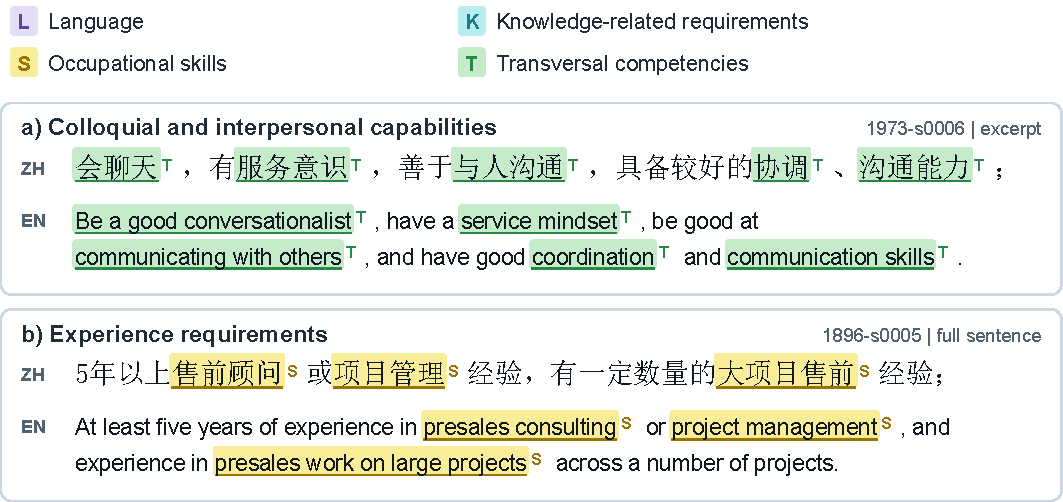
\includegraphics[width=\linewidth]{figures/annotation_examples_additional_20261006.pdf}
\caption{Additional human-reference examples with aligned English translations. Chinese highlights retain the frozen reference spans (v4.2.10 metadata); matching colors and labels identify their English counterparts.}
\label{fig:additional-annotation-examples}
\end{figure}

\FloatBarrier
% [R16-B] Preserve original comparison layers; administrative provenance stays in archived sources.
\section{Appendix B. Annotation-Quality Evidence}
\phantomsection
\label{app:b}
\label{sec:quality-provenance-r12}
We describe reference construction, assisted review, and the separate blinded study (Table~\ref{tab:quality-main}).

\subsection{Human Annotation and Review Coverage}
\label{sec:human-review-coverage}
The 150-sentence human reference, initial 100-sentence silver review, and separate 100-sentence post-generation review cover 350 unique sentences. The early 15-sentence assisted-review subset is included in the post-generation cohort. The additional review contributes 150 sentences: 60 cloud, 45 public-sector, and 45 listed-company sentences. Identifier and normalized-text checks excluded the original 350 sentences from this additional sample, yielding 500 sentences with human annotation or review before the blinded study. The 50-sentence blinded study has no normalized-text overlap with these cohorts, bringing coverage to 550 distinct sentences. Each sentence is counted once across annotation layers. Model-evaluation labels come from the 150-sentence human reference; the remaining cohorts serve annotation-quality assessment.

\subsection{Reference Construction and Initial Agreement}
The human reference combines 50 calibration sentences sampled from the 980-record model-disagreement queue and a separate 100-sentence challenge sample. The calibration sentences were annotated separately and adjudicated; the challenge sample was collaboratively annotated and reviewed. The authors recall machine suggestions being available during calibration, whereas an earlier protocol specifies raw-text-only coding. The available records do not resolve this discrepancy, so this stage is not treated as a blinded agreement study. All 50 calibration sentence IDs are absent from the silver training and development sets.

The finalized reference contains 415 challenge-sample spans (290 S, 83 K, 41 T, one L) and 248 calibration-sample spans (158 S, 42 K, 47 T, one L). Seven challenge sentences and one calibration sentence have no annotated span. The 150 reference sentences correspond to 61 source-document prefixes in the original corpus. These reference labels are used for model evaluation and remain separate from the individual coding and assisted-review layers.

The two available calibration annotation layers contain 211 and 230 spans, with 98 exact typed matches and F1 of 0.444. Character-level $\kappa$ is 0.567 across all 2,571 source code points, including spaces and punctuation. These retrospective estimates use available exports whose correspondence to the original frozen files has not been verified. They describe initial agreement, rather than an independent assessment of the adjudicated reference. Comparisons with that reference involve the same annotators and reflect adjudication changes; the detailed scores and supporting records are provided in the \href{https://github.com/AlfredJamesLi/chinese-skillspan-benchmark/blob/main/reproduction/annotation_documentation_20261007/README.md}{annotation documentation}.

% [R37-MOVE] Counting convention formerly repeated in the corpus chapter.
Character-level Cohen's $\kappa$ adjusts observed agreement for agreement expected by chance from the two coders' marginal label frequencies across the source character positions:
\begin{equation}
\kappa=\frac{p_o-p_e}{1-p_e},
\qquad p_e=\sum_{c\in\mathcal{C}}p_A(c)\,p_B(c).
\label{eq:character-kappa}
\end{equation}
Here, $p_o$ is the fraction of source character positions with identical labels, and $p_A(c)$ and $p_B(c)$ are the two coders' label proportions. The label set $\mathcal{C}$ comprises L/K/S/T and O. For the four-label scheme plus O, the available exports yield $p_o=0.771$ and $p_e=0.471$, giving $\kappa=0.567$. These coefficients use character positions rather than the spans counted in Eq.~\eqref{eq:micro-prf}. The 2,571 positions are nested within the 50 sampled sentences.

When both annotations of a sentence are empty, the pair contributes no span true positives. Span matching and character-level agreement use different units; optional category projections are described in the reproduction materials.

\subsection{Post-Generation Assisted Review}
The 100-sentence post-generation review sample was stratified by source, empty/nonempty annotation, and text length. The sampling frame contained 2,179 eligible records after excluding 100 initially reviewed records, 100 reserved for an earlier pilot, and 72 pending records from the 2,451-record original silver pool. Two small strata totalling 11 records were unsampled.

Comparing machine-prefilled and human-reviewed annotations yields 140 exact typed matches among 144 machine and 148 reviewed spans: precision is 0.972, recall 0.946, and F1 0.959. Ninety-five sentences have identical span sets. These estimates apply to this stratified sample.

The 15-sentence assisted-review subset is nested within the post-generation Silver review cohort. Both annotators had access to machine coding suggestions. Their human layers contain the same 27 spans, yielding exact span F1 and character kappa of 1.000. The shared suggestions may contribute to this agreement between assisted reviewers.

\subsection{Supervision Counts and Length Summaries}
Figure~\ref{fig:length-distributions-r40} compares the supervision and human-reference distributions. The median input length is 33 Unicode code points in the silver training and development sets used by Qwen and the encoders, and 41.5 in the human reference. Median span lengths are six and four code points, respectively. The training and development sets contain 3,646 and 345 spans; 869 of 2,150 training records (40.4\%) and 82 of 169 development records (48.5\%) have no annotated span. Table~\ref{tab:expanded-silver-composition} reports record counts, including repetitions, for the full adopted expanded pool and its Qwen splits.

\begin{table}[htbp]
\caption{Competency-span counts in the adopted expanded Silver pool and its Qwen splits.}
\label{tab:expanded-silver-composition}
\centering\small
\setlength{\tabcolsep}{4pt}
\begin{tabular}{@{}lrrrrrrr@{}}
\toprule
Split & Records & \makecell{Empty annotations\\$n$ (\%)} & L & S & K & T & Total spans \\
\midrule
Training & 8,842 & 2,321 (26.2\%) & 149 & 10,653 & 4,887 & 3,851 & 19,540 \\
Validation & 348 & 91 (26.1\%) & 2 & 403 & 184 & 152 & 741 \\
Test & 350 & 80 (22.9\%) & 4 & 472 & 194 & 150 & 820 \\
\midrule
Full pool & 9,540 & 2,492 (26.1\%) & 155 & 11,528 & 5,265 & 4,153 & 21,101 \\
\bottomrule
\end{tabular}
\par\smallskip
{\footnotesize\RaggedRight Percentages use the number of records in each split.\par}
\end{table}

\FloatBarrier

\subsection{Additional Review of Newly Generated Silver Labels}
In the additional assisted review, two reviewers separately annotated the same 150 sentences with Codex and Cursor suggestions visible (Table~\ref{tab:annotation-models}). Figure~\ref{fig:additional-review-distributions} shows their shared input-length distribution and separate span-length distributions. Median input length is 33.5 Unicode code points; both reviewers' median span length is six, with maxima of 41 for A and 42 for B. Lengths include spaces and punctuation, and the input distribution includes sentences with empty annotations.

\begin{figure}[!htbp]
\centering
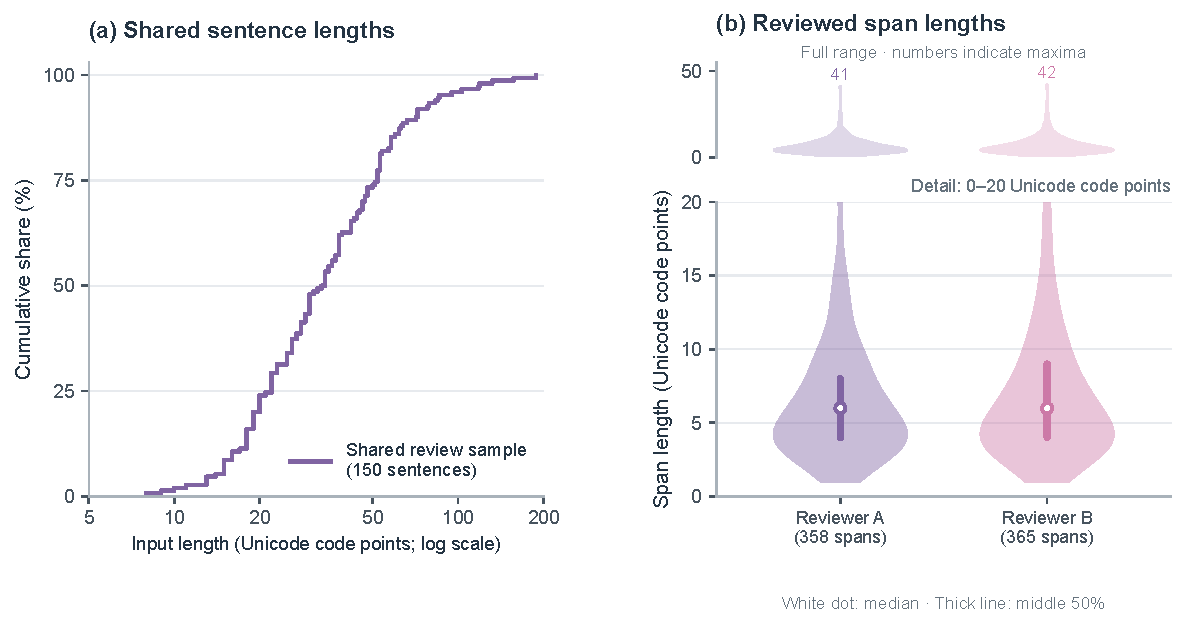
\includegraphics[width=\linewidth]{figures/additional_review_profile_20261006.pdf}
\caption{Length distributions in the additional assisted-review sample. Panel (a) uses the same 150 sentences for both reviewers; panel (b) shows their separate annotation layers, with 358 spans for A and 365 for B. Densities use all observed spans with equal maximum widths. The overview shows the full range of span lengths, while the detail view focuses on 0--20 Unicode code points. Dots mark medians, and thick lines mark the middle 50\%. Supervision and human-reference distributions appear in Figure~\ref{fig:length-distributions-r40}; reviewer-specific type counts appear in Table~\ref{tab:additional-review-composition}.}
\label{fig:additional-review-distributions}
\end{figure}

Table~\ref{tab:additional-review-composition} gives both reviewers' type counts. Table~\ref{tab:qa150-pairs} compares pre-adjudication span sets. Its 95\% percentile intervals use 10,000 sentence resamples within source strata, with source quotas fixed.

\begin{table}[htbp]
\caption{Competency composition in the additional review sample: span counts (within-reviewer percentages).}
\label{tab:additional-review-composition}
\centering\small
\begin{tabular}{@{}lrrrrr@{}}
\toprule
Reviewer & L & S & K & T & Total spans \\
\midrule
A & 3 (0.8\%) & 217 (60.6\%) & 77 (21.5\%) & 61 (17.0\%) & 358 \\
B & 3 (0.8\%) & 218 (59.7\%) & 81 (22.2\%) & 63 (17.3\%) & 365 \\
\bottomrule
\end{tabular}
\end{table}

\begin{table}[htbp]
\caption{Typed exact-span agreement in the additional review sample.}
\label{tab:qa150-pairs}
\centering\small
\begin{tabularx}{\linewidth}{@{}Lccc@{}}
\toprule
Comparison & Exact F1 & 95\% CI & \makecell{Sentences with\\identical span sets} \\
\midrule
Reviewer A--Reviewer B & 0.816 & [0.769, 0.860] & 101/150 \\
Codex--Cursor suggestions & 0.962 & [0.937, 0.983] & 138/150 \\
Reviewer A--Codex suggestions & 0.823 & [0.776, 0.866] & 100/150 \\
Reviewer B--Codex suggestions & 0.850 & [0.803, 0.892] & 108/150 \\
\bottomrule
\end{tabularx}
\par\smallskip\footnotesize\RaggedRight
F1 is micro-averaged; CIs are 95\% percentile intervals from a source-stratified sentence bootstrap.
\end{table}

Agreement uses both reviewers' complete annotation layers, including the 49 sentences with differing span sets. Character-level calculations assign O/L/K/S/T to the original Unicode-code-point positions, including spaces and punctuation. Two positions have conflicting types within one reviewer's layer; excluding them from both character sequences leaves $N=5{,}990$ positions. All original spans remain in span-level F1. The accompanying agreement data identify the affected record. Later adjudication and incorporation into training targets have not been verified. Agreement over the retained character positions is $p_o=0.934$, with $p_e=0.439$ and $\kappa=0.883$.

For nominal Krippendorff's $\alpha$, let $m_c$ count assignments to category $c$ across both reviewers, with $\sum_c m_c=2N$. The observed and expected disagreements are
\begin{equation}
\alpha=1-\frac{D_o}{D_e},\qquad
D_o=1-p_o,\qquad
D_e=1-\frac{\sum_c m_c(m_c-1)}{2N(2N-1)}.
\label{eq:qa150-alpha}
\end{equation}
Here $D_o=0.066$ and $D_e=0.560$, giving $\alpha=0.883$. Character coefficients include the many O positions, whereas span F1 assesses complete spans~\citep{artstein2008agreement}. The machine--machine comparison measures concordance between the suggestion layers.

\subsection{Blinded Coding by Three Annotators}
The annotators were one human resource management specialist with a doctorate and two working professionals pursuing master's degrees in management. The students had sustained annotation experience and three to five years of professional experience. All three contributed to handbook development; two professors advised on the coding process and handbook preparation.

The formal sample comprises eight listed-company, 16 public-institution, and 26 Tianchi sentences from the silver annotation candidates, with one sentence per advertisement identifier. The team reports random selection, although the candidate frame and sampling log are unavailable; the released annotations identify the sampled sentences and sources. Preparation used five familiarization and 15 practice sentences, all excluded from the agreement analysis. The available records do not establish whether all annotators followed the same sequence.

\begin{sloppypar}
The annotators coded independently and could review their own labels using the study handbook, with machine suggestions and other annotators' labels hidden throughout. The main analysis uses each annotator's individual annotations after self-review, as confirmed by the authors, and includes all 50 sentences and all annotator pairs. Mean pairwise typed exact-span F1 is 0.818; the annotations were not adjudicated into a consensus reference. Earlier individual annotations yielded 0.663. Both sets are available in the \href{https://github.com/AlfredJamesLi/chinese-skillspan-benchmark/tree/main/reproduction/style_revision_20261005}{reproduction notes}, but the recorded timing does not establish a comparable before-and-after sequence across annotators. \hyperref[sec:guide-version-history]{Appendix A.4} distinguishes the handbook records from later reader editions. The sample overlaps with expanded-model training data (\hyperref[app:d]{Appendix D}); historical model-reference labels remain unchanged.
\end{sloppypar}

Annotators A, B, and C produced 104, 123, and 113 spans, respectively. Exact typed matches number 90 for A--B, 92 for A--C, and 96 for B--C. O covers 63.2--64.1\% of character positions.

% Detailed blinded-agreement evidence relocated from the corpus chapter.
\phantomsection
\label{sec:blinded-agreement-details}

For typed exact-span F1, a match requires identical boundaries and types, and the two annotators are treated symmetrically~\citep{hripcsak2005agreement}. Boundary-only exact-span F1 ignores type. Character-level agreement uses pairwise Cohen's $\kappa$ and three-annotator nominal Krippendorff's $\alpha$ on L/K/S/T/O assignments to all 2,111 source Unicode code points; O denotes positions outside annotated spans. Character-level coefficients summarize agreement at each position, while span-level F1 requires complete span matches~\citep{artstein2008agreement}.

The 95\% percentile confidence intervals use 10,000 sentence-bootstrap samples drawn within source strata, with all three annotation layers retained together for each sampled sentence. They summarize variation within the sampled strata for these three annotators. Table~\ref{tab:blinded-agreement-pairs} gives the pairwise comparisons underlying Table~\ref{tab:quality-main}.

\begin{table}[!htbp]
\caption{Pairwise agreement on the 50-sentence blinded sample after individual self-review.}
\label{tab:blinded-agreement-pairs}
\centering\small
\setlength{\tabcolsep}{4pt}
\begin{tabularx}{\linewidth}{@{}P{.14\linewidth}P{.26\linewidth}P{.22\linewidth}P{.16\linewidth}L@{}}
\toprule
Pair & Typed exact F1 [95\% CI] & Boundary-only exact F1 & Cohen's $\kappa$ & \makecell[l]{Identical\\span sets\\(sentences)} \\
\midrule
A--B & 0.793 [0.694, 0.884] & 0.828 & 0.880 & 36/50 \\
A--C & 0.848 [0.752, 0.926] & 0.876 & 0.930 & 39/50 \\
B--C & 0.814 [0.721, 0.899] & 0.847 & 0.909 & 37/50 \\
\bottomrule
\end{tabularx}
\par\smallskip
{\footnotesize\RaggedRight F1 compares complete spans; identical span sets include empty sets. Cohen's $\kappa$ uses L/K/S/T/O labels at source character positions. CIs are 95\% percentile confidence intervals.\par}
\end{table}

Mean pairwise typed exact-span F1 was 0.818 (95\% CI [0.732, 0.894]), and boundary-only exact-span F1 was 0.850 (95\% CI [0.766, 0.923]). By type, pairwise F1 ranges were 0.762--0.805 for K, 0.778--0.869 for S, and 0.865--1.000 for T. Character-level $\alpha$ was 0.907 (95\% CI [0.851, 0.954]).

All three annotators produced identical complete typed-span sets for 34 sentences, including 11 with no annotated spans. They also identified the same two L spans, both in one sentence, providing limited evidence about agreement on this category. Individual annotation exports and diagnostics are available in the \href{https://github.com/AlfredJamesLi/chinese-skillspan-benchmark/tree/main/reproduction/agreement/finalguide_abc_20261003}{reproduction materials}.


\subsection{Silver Labels against Blinded Annotations}
We compared the final expanded-pool labels with each of the three blinded annotation layers on the same 49 retained sentences (Table~\ref{tab:silver-blinded}). One of the 50 study sentences remained unresolved at the candidate stage and was absent from both final pools; it was excluded from this comparison rather than scored as an empty annotation. Each per-annotator score pools exact boundary-and-type matches across the 49 sentences, and the mean averages the three micro-F1 scores.

\begin{table}[!htbp]
\centering\small
\caption{Agreement between final expanded Silver labels and individual blinded annotations.}
\label{tab:silver-blinded}
\begin{tabularx}{\linewidth}{@{}Lrrrrr@{}}
\toprule
Silver pool & Sentences & Annotator A & Annotator B & Annotator C & Mean \\
\midrule
Adopted expanded pool & 49 & 0.724 & 0.681 & 0.721 & 0.709 \\
Alternative expanded pool & 49 & 0.723 & 0.716 & 0.721 & 0.720 \\
\bottomrule
\end{tabularx}
\par\smallskip\footnotesize\RaggedRight
Values are typed exact-span micro-F1; the mean is taken across annotators A--C.
\end{table}

This post hoc analysis compares historical silver labels with human annotations made without access to machine suggestions. It complements the assisted reviews, but its findings apply to the selected sample and participating annotators and do not estimate accuracy across the full silver pool. Counts, input hashes, and code are provided in the \href{https://github.com/AlfredJamesLi/chinese-skillspan-benchmark/tree/main/reproduction/reviewer_revision_20261005}{reproduction materials}. The original 150-sentence model scores are unchanged.

\FloatBarrier

% Current evaluation evidence retained; historical studies archived in reproduction/supplementary_tables.
\section{Appendix C. Supplementary Evaluation}
\phantomsection
\label{app:c}
This appendix covers the shared protocol, uncertainty, errors, the JobBERT supervision comparison, and exploratory expanded-pool results. The \href{https://github.com/AlfredJamesLi/chinese-skillspan-benchmark/blob/1d1c24e20ee049fc768034b5baf58fa882e08e2c/reproduction/process_archive_20260924/secondary_review/README.md}{supporting records} give per-run results, scorer details, and earlier protocol comparisons across output formats and demonstration settings.

\subsection{Detailed Human-Reference Model Results}
Tables~\ref{tab:gold150-shared-r7}, \ref{tab:gold150-main}, and \ref{tab:external-chinese} complement Figure~\ref{fig:model-comparison} with detailed model and type-specific scores.

\input{tex/stage2_shared_main}

\begin{table}[!htbp]
\caption{Human-reference results for Qwen adaptation and silver-trained JobBERT.}
\label{tab:gold150-main}
\centering\small
\textbf{A. Qwen: fixed inference protocol}\par\smallskip
\begin{tabularx}{\linewidth}{@{}Lcccc@{}}
\toprule
Condition & \makecell{Train / dev\\records} & Typed exact & Typed relaxed & \makecell{Boundary-only\\exact} \\
\midrule
No adapter & --- & $\QwenBaselineExact$ & $0.470$ & $0.414$ \\
Qwen + LoRA & 2,150 / 169 & $\QwenLoraExact$ & $0.662\pm0.033$ & $0.571\pm0.038$ \\
\bottomrule
\end{tabularx}
\par\medskip\textbf{B. Silver-trained JobBERT baseline}\par\smallskip
\begin{tabularx}{\linewidth}{@{}Lcc@{}}
\toprule
Model & \makecell{Train / dev\\records} & Typed exact \\
\midrule
JobBERT-zh + CRF & 2,156 / 169 & $0.554\pm0.005$ \\
\bottomrule
\end{tabularx}
\par\smallskip\footnotesize\RaggedRight
Micro-F1: mean $\pm$ sample SD (seeds 42, 43, 44); unadapted Qwen: single run. Boundary-only F1 ignores type.
\end{table}

\FloatBarrier


% [R42] Final A handoff, independently rescored; old snapshot preserved in before_R42.
% Separate protocol: no changes to the abstract or historical V4 result.
\subsection{Shared-Guideline Evaluation against the Human Reference}
\label{sec:gold150-shared-r7}
The shared protocol evaluates six configurations on all 150 reference sentences, using V4.2.12-based general instructions and five schematic examples.

\paragraph{Configuration and output records.}
Table~\ref{tab:model-identity} distinguishes the original annotation teacher, inference baselines, and expansion channels, with their recorded identifiers and access configurations.

\input{tex/review20260923/model_identity}

Models return an ID and spans as literal \texttt{text}, zero-based \texttt{occurrence}, and L/K/S/T \texttt{type}. The span parser resolves spans to Unicode offsets for exact and relaxed scoring with the released span scorer. All supplied input texts match the frozen reference.

Qwen uses deterministic decoding; Kimi uses non-thinking mode at temperature 0.6. DeepSeek output caps are 2,048 tokens without thinking and 8,192 with thinking. Access routes appear in Table~\ref{tab:model-identity}; full configurations accompany the reproduction notes.

\paragraph{Parser and matching conventions.}
The parser resolves literal spans to source offsets, sorts candidates by start offset and original output order, and keeps the first compatible candidate. Later duplicates, same-boundary type conflicts, and overlaps are rejected. Partial responses retain accepted spans; fully rejected or malformed responses become empty predictions. Identifier coverage is checked across all supplied sentences before scoring.

Exact matching deduplicates identical span tuples within each sentence. Relaxed matching traverses reference spans in source order and selects the unused same-type prediction with highest IoU, taking the first prediction on a tie. The threshold is 0.5, and matching is greedy rather than globally optimized. Empty--empty records contribute no span counts. The \href{https://github.com/AlfredJamesLi/chinese-skillspan-benchmark/blob/1d1c24e20ee049fc768034b5baf58fa882e08e2c/reproduction/process_archive_20260924/secondary_review/source/tex/appendix_C_shared_R16.tex}{scorer specification} preserves schema validation, BIO edge cases, and executable checks. The sentence-level counts reproduce the published exact scores before resampling.

\paragraph{Conditional resampling.}
To allow dependence among sentences with the same source identifier, we grouped the 150 reference sentences by the prefix preceding \texttt{-s}, giving 61 groups. Each of 10,000 paired bootstrap draws samples 61 complete groups with replacement and includes all their sentences. The same draw is used for all compared models and each fixed training seed; micro-F1 is recomputed before seed means and paired differences are calculated. Table~\ref{tab:core-paired} reports percentile intervals. The prefixes agree with the stored source-document identifiers in the original corpus. Group resampling accounts for dependence among sentences from the same document; it does not change split membership. These secondary intervals condition on the selected reference and trained models, and are not adjusted for multiple comparisons. The reproduction package retains the earlier sentence-bootstrap results and the seed used for the group analysis. Training-seed SD measures a separate source of variation. As a sensitivity check, widening the bootstrap intervals for the six displayed comparisons using Bonferroni tail probabilities leaves all inclusion/exclusion-of-zero conclusions unchanged; detailed intervals and code are in the supplementary calculations.

\paragraph{Observed mismatch examples.}
In the frozen no-adapter Qwen output for \texttt{1801-s0004}, the predicted S span $[5,24)$ is \zh{参与公司无人机飞控系统技术项目开发策划} (\emph{participate in planning a technical development project for the company's UAV flight-control system}), whereas an overlapping reference S span is $[16,24)$, \zh{技术项目开发策划} (\emph{technical project development planning}). For \texttt{1802-s0005}, both layers select \zh{方法} (\emph{method}) at $[6,8)$, but the prediction is S and the reference is K. These frozen outputs illustrate boundary and type mismatches with the reference; they have not been separately adjudicated. After removing exact matches, the pairing procedure identifies 27 same-boundary/different-type pairs, 89 same-type/overlapping-boundary pairs, and 65 other unmatched predictions, totalling 181 false positives. These counts classify span relationships rather than linguistic causes. The \href{https://github.com/AlfredJamesLi/chinese-skillspan-benchmark/blob/1d1c24e20ee049fc768034b5baf58fa882e08e2c/reproduction/process_archive_20260924/secondary_review/source/tex/appendix_C_shared_R16.tex}{error-analysis data} records the pairing order and parser errors; a full adjudicated error taxonomy remains unavailable.

\FloatBarrier
The released predictions and scoring code reproduce the reported exact and relaxed scores.

Under their respective output budgets, DeepSeek in thinking mode has higher precision and lower recall than the recorded non-thinking configuration.

\paragraph{Per-seed Qwen results.}
\label{sec:qwen-shared-sft-r42}
The \href{https://github.com/AlfredJamesLi/chinese-skillspan-benchmark/blob/1d1c24e20ee049fc768034b5baf58fa882e08e2c/reproduction/process_archive_20260924/secondary_review/README.md#previous-table-17-qwen-per-seed-and-cohort-scores}{per-seed record} retains precision, recall, exact/relaxed F1, and calibration/challenge scores underlying Tables~\ref{tab:gold150-main} and \ref{tab:core-paired}. Boundary exact F1 in Table~\ref{tab:gold150-main} was subsequently recomputed from the same frozen accepted spans, with types collapsed and duplicate coordinates removed within sentences. This adds a scoring view without new training or inference. The \href{https://github.com/AlfredJamesLi/chinese-skillspan-benchmark/tree/main/reproduction/model_diagnostics_20261003}{model-diagnostic records} provide per-seed and per-type precision, recall, TP/FP/FN, and the full-precision summaries used in Table~\ref{tab:external-chinese}; Figure~\ref{fig:qwen-diagnostics} retains individual-seed Qwen results.
\FloatBarrier
\subsection{Qwen Prediction Diagnostics}
\label{sec:qwen-diagnostics-r2}

Figure~\ref{fig:qwen-diagnostics} reuses the same 150 reference sentences and the accepted spans from each run. Typed exact matching is completed on each full sentence before aggregation by reference-span length. Bins ($\leq4$, 5--8, $\geq9$ Unicode code points) are fixed in advance; they contain 346/243/74 reference spans in 102/110/56 sentences, respectively. A sentence may contribute reference spans to multiple bins. Type-specific unmatched predictions count as FP even in empty-reference sentences. Results for each training seed are evaluated separately on the same reference sentences.

On the eight empty-reference sentences, accepted false-positive spans decrease from 19 without an adapter to 6, 4, and 0 for seeds 42, 43, and 44; affected sentences number 2, 2, 1, and 0.

L has two reference spans: the no-adapter run recovers 0/2 and each LoRA run 2/2, with one extra L prediction in every run. Complete TP/FP/FN, legal-empty-output counts, and parser-rejection diagnostics are available in the \href{https://github.com/AlfredJamesLi/chinese-skillspan-benchmark/blob/1d1c24e20ee049fc768034b5baf58fa882e08e2c/reproduction/process_archive_20260924/secondary_review/source/tex/qwen_diagnostics_round2.tex}{diagnostic records}.

\subsection{JobBERT under Different Label Versions}
\label{sec:jobbert-label-versions}

\paragraph{Supervision and model selection.} The two JobBERT conditions start from the same released encoder and inherited CRF. Earlier supervision (archived as \texttt{B1}) uses historical extraction labels, whereas revised supervision (archived as \texttt{B2}) incorporates updated guidelines, LLM annotations, and adjudication. The conditions use the same training and development texts, with label changes in 1,440 training records and 107 development records. Checkpoints are selected by typed exact-span F1 against the corresponding development labels. The comparison therefore changes both training supervision and checkpoint-selection targets. Both conditions use the JobBERT training settings in Table~\ref{tab:training-settings}. The revised-label condition is the Silver-trained JobBERT-zh + CRF baseline reported in the main results. Qwen and the encoder comparison use 2,150 training and 169 development records with revised labels, after the exclusions described in \nameref{sec:experiments}. These sets differ from JobBERT's 2,156/169 inputs and the original 2,451-record Silver candidate pool.

\begin{table}[htbp]
\centering\small
\caption{JobBERT performance with earlier and revised labels on matched texts.}
\label{tab:jobbert-label-versions}
\begin{tabularx}{\linewidth}{@{}Lcc@{}}
\toprule
Label version & \makecell{Train / dev\\records} & Typed exact \\
\midrule
Earlier labels & 2,156 / 169 & $0.142\pm0.014$ \\
Revised labels & 2,156 / 169 & $0.554\pm0.005$ \\
\bottomrule
\end{tabularx}
\par\smallskip\footnotesize\RaggedRight
Typed exact-span micro-F1 on the human reference set; mean $\pm$ sample SD over seeds 42, 43, and 44. Both training labels and checkpoint-selection labels differ between conditions.
\end{table}

The revised-label setting has higher human-reference F1 than the earlier-label setting (Table~\ref{tab:jobbert-label-versions}).

% Verified against GitHub commit 11355ff and the author-supplied Server A README.
\subsection{Exploratory Expanded-Silver Experiments}
\label{sec:expanded-silver}
The expanded Qwen experiments use 8,842/348/350 training/validation/test records from the adopted silver pool and 8,943/351/352 from the alternative pool. Both combine earlier supervision with additional annotations and differ in annotation channel and included records. Shared records retain their split assignments. Checkpoints are selected by typed exact-span F1 on silver validation labels. The silver tests use separate sentence splits whose source-document groups overlap with training. Fitting and model selection exclude human-reference sentences (\hyperref[app:d]{Appendix D}).

The expanded Qwen runs use seed 42, the shared prompt and parser, the output format based on span text and occurrence indices, and the training settings in Table~\ref{tab:training-settings}. The loss is computed only over the assistant's output. Training uses early stopping with a patience of two epochs. Both Qwen checkpoints are selected at epoch one by exact F1 on the silver validation set; decoding is deterministic with a 2,048-token output cap. Full settings are available in the \href{https://github.com/AlfredJamesLi/chinese-skillspan-benchmark/blob/1d1c24e20ee049fc768034b5baf58fa882e08e2c/reproduction/process_archive_20260924/secondary_review/source/tex/expanded_silver_results_20260917.tex}{experiment archive}. The expanded JobBERT runs retain the domain-adapted encoder and inherited CRF. The adopted-pool JobBERT run uses 8,842 training and 698 development records. Qwen instead uses 348 validation and 350 test records with the same 8,842-record training set.


\begin{table}[htbp]
\caption{Expanded-pool Qwen results (seed 42).}
\label{tab:expanded-silver-main}
\centering\small
\begin{tabularx}{\linewidth}{@{}Lcccc@{}}
\toprule
Pool variant & \makecell{Silver validation\\agreement} & \makecell{Silver test\\agreement} & \makecell{Human reference\\exact} & \makecell{Human reference\\relaxed} \\
\midrule
Alternative & 0.783 & 0.759 & 0.597 & 0.713 \\
Adopted & 0.833 & 0.809 & 0.585 & 0.703 \\
\bottomrule
\end{tabularx}
\par\smallskip\footnotesize\RaggedRight
Typed span micro-F1 (exact unless marked relaxed). Training/validation/test sizes: alternative, 8,943/351/352; adopted, 8,842/348/350.
\end{table}

The annotation-channel comparison replaces a 2,500-candidate batch (Table~\ref{tab:source-stages}). The adopted-pool configuration has higher agreement with its silver test labels but a lower observed exact F1 on the human reference than the alternative-pool configuration. The replaced batch contains 2,353 accepted Codex annotations and 2,459 accepted annotations obtained through the API, respectively. The score difference thus reflects changes in both labels and included records.

On the human reference set, expanded JobBERT obtains exact F1 of 0.242 with the alternative pool and 0.232 with the adopted pool (seed 42); the latter has relaxed F1 of 0.485. A separate configuration trained on 7,117 newly annotated records gives $0.237\pm0.002$ across three seeds. All are below the original Silver-trained JobBERT-zh + CRF result. Alongside training size, these experiments change the annotation protocol, source composition, and development set.

For comparison, Qwen trained on the original 2,150-record Silver set scores 0.500 at seed 42 and averages 0.540 across three seeds. Expanded-pool Qwen therefore scores higher in these runs, whereas expanded JobBERT scores lower. Because supervision and checkpoint-selection targets change together, the results support an exploratory comparison of complete configurations. Further controlled experiments are needed to explain the JobBERT decline, including possible effects of label versions, input windowing, and decoding.

The \href{https://github.com/AlfredJamesLi/chinese-skillspan-benchmark/blob/36f009fab01b8433355cb7ef5af8fad02c6cc519/reproduction/process_archive_20260924/README.md}{supplementary materials} report exploratory single-seed supervision-subset experiments with different checkpoint-selection rules.

\section{Appendix D. Data Lineage, Access, and Reproduction}
\phantomsection
\label{app:d}
\label{sec:extension-provenance}
\label{sec:display-archive-r14}

Data Availability and Table~\ref{tab:component-access} summarize the released materials and access conditions. The \href{https://github.com/AlfredJamesLi/chinese-skillspan-benchmark/tree/main/reproduction/major_revision_20261004}{supplementary audit package} provides supporting calculations and archived experiment records.

\begin{samepage}
The terms \texttt{Gold150}, \texttt{QA150}, and \texttt{Silver-plus} denote the human reference, additional review sample, and original silver candidate pool, respectively. The main silver-supervised baselines use model-specific training/development subsets of this pool with revised labels (\hyperref[sec:jobbert-label-versions]{Appendix C}).\par
\end{samepage}

\subsection{Relationship to the Earlier Preprint}
The present article substantially revises the resource definitions, annotation procedures, and evaluations in the earlier preprint~\citep{li2026chineseskillspanpreprint}. The sample list and original annotations for the earlier 100-sample agreement report have not been recovered, so those results are not used to establish reliability for the present reference. The available experiment records do not substantiate the earlier descriptions of linking spans to concepts or evaluating on industries and time periods excluded from training. The current article therefore makes neither claim. Model results use the reference labels, supervision sets, and scoring procedures documented for each experiment.

\subsection{Source Categories and Data Preparation}
The source corpus was originally partitioned into 17,460 training, 2,143 development, and 3,237 test sentences, with 1,600, 200, and 200 source-document identifiers, respectively. These document-disjoint partitions describe the source corpus; the original test partition is not a human-annotated evaluation set in this study. Tianchi material came from the Recruitment Dataset (ID 163746). The public-institution crawler revisited selected pages weekly or monthly.

The initial annotation collection contains 2,601 records: 150 human-reference sentences and 2,451 original silver records. The silver pool comprises 100 initially reviewed records, 730 additional records from the model-disagreement queue, and 1,621 historical extraction records. The 980-record queue supplied the 150-sentence human reference and the first 830 silver records. Model-specific inclusion rules produce the supervision splits described in \nameref{sec:experiments}.

The corpus combines four batches collected through MacroData, public-institution websites, and Tianchi. The original training partition contains 10,312 graduate-recruitment sentences and 7,148 sentences from the AI collection; development contains 2,143 sentences from the AI collection; test contains 1,423 from the AI collection, 473 from Tianchi/cloud, and 1,341 from public institutions. The expanded data use three source categories: Tianchi/cloud, public institutions, and listed companies. The blinded sample contains 26, 16, and 8 sentences from these respective categories.

MacroData's operator is Chongqing Maherui Information Technology Co., Ltd. Public-institution records retain source names, titles, URLs, listed publication dates, and geographic fields where available. Publication dates are not collection dates; a complete crawl-window and source-exclusion history has not been recovered. The authors confirm academic-research use permission. Repository notices distinguish author-created annotation rights from third-party text restrictions.

Table~\ref{tab:source-stages} gives expanded-pool candidate and retained counts. Intermediate preparation counts are documented in the \href{https://github.com/AlfredJamesLi/chinese-skillspan-benchmark/tree/main/reproduction/reviewer_revision_20261005}{preparation memo}.

\begin{table}[!htbp]
\centering\small
\caption{Recovered sampling-stage counts and missing census information. These are sentence counts, not advertisement counts or mutually exclusive industry totals.}
\label{tab:source-stages}
\begin{tabularx}{\linewidth}{@{}P{.25\linewidth}P{.26\linewidth}L@{}}
\toprule Stage & Available counts & Sampling frame / unavailable detail \\
\midrule
Original four collections & 22,840; split 17,460/2,143/3,237 & AI, Cloud, public-sector, graduate recruitment. Per-source ad counts, time windows, attrition and complete document mapping not recovered. \\
Targeted study lineage & 980 conflict-origin + 1,621 other records & 150 reference + 2,451 Silver-plus. This is a selected lineage, not a probability sample. \\
New expansion candidates & Cloud 3,174; public-sector 2,381; listed-company 2,381 & Requirement-keyword-positive sentences; fixed hash ranking. Earlier B2 contributes 2,064 retained unique sentences. \\
Replacement channel subset & 2,500 candidates; alternative retains 2,459; Codex retains 2,353 & Respective exclusions: 41 (1.6\%) and 147 (5.9\%). A reason-coded attrition breakdown is not established. \\
Additional QA150 & 60 / 45 / 45 source quotas & Sampled from new Silver; machine suggestions visible. Does not extend the independent test population. \\
\bottomrule
\end{tabularx}
\end{table}


New sentences were selected using requirement-related keywords, a fixed hash-based order for selecting candidates, and quotas for each source. Before annotation, the texts were cleaned for HTML markup and whitespace, split into sentences, and filtered by length. Checks for excluding previously used texts relied on the stored sentences and available pretraining data. No checksum was retained for the 3.2-million-line pretraining file, so the data seen during pretraining cannot be fully reconstructed. Earlier annotations have been preserved; the available records identify the prompts and handbook versions for each documented batch (\hyperref[sec:guide-version-history]{Appendix A.4}).

\subsection{Split Membership and Document Overlap}
The later experiments divide the data by sentence, whereas the original 22,840-sentence corpus was divided so that each source document appeared in only one split. Original records identify source documents; records added during expansion identify source files and rows. The two identifier systems have not been linked, so shared sources can be checked only within each system. Qwen and the encoders use 2,150 original silver records for training and 169 for development.

\begin{table}[htbp]
\centering\small
\caption{Shared source-document groups in the later experimental splits.}
\label{tab:document-overlap}
\begin{tabularx}{\linewidth}{@{}Lrrr@{}}
\toprule Split comparison & Shared groups & \makecell{Records in\\first split} & \makecell{Records in\\second split} \\
\midrule
Silver train / development & 1 & 4 & 27 \\
Silver train / human reference & 59 & 531 & 143 \\
Silver development / human reference & 0 & 0 & 0 \\
Adopted expanded train / validation & 185 & 1,060 & 208 \\
Adopted expanded train / test & 188 & 1,076 & 210 \\
Alternative expanded train / validation & 186 & 1,069 & 210 \\
Alternative expanded train / test & 189 & 1,079 & 211 \\
\bottomrule
\end{tabularx}
\par\smallskip\footnotesize\RaggedRight
Counts refer to sentence records in shared source-document groups; records with different identifiers are counted separately even when their text is identical. Split order follows the first column.
\end{table}

We checked for repeated sentence texts across splits by comparing complete texts as stored and after Unicode NFC normalization, which gives equivalent Unicode character sequences a consistent representation. Neither comparison found matching texts between the original silver training and development sets used by Qwen and the encoders, or between training and the human reference.

A broader check used Unicode NFKC normalization, which also standardizes forms such as full-width and half-width characters, then removed whitespace and ignored letter case. This check found no matching complete texts between the original silver training set and the human reference. It found two training/development matches in the original silver data and one training/validation match in each expanded pool, with no training/test matches in either expanded pool. These checks compare texts without changing the stored sentences or annotation offsets; details are provided in the \href{https://github.com/AlfredJamesLi/chinese-skillspan-benchmark/blob/24847748b314b205e9b896c1f30ecc5d7c7bdf1e/reproduction/major_revision_20261004/data_audit/audit.json}{text-overlap analysis}. Table~\ref{tab:document-overlap} reports shared source-document groups separately.

The silver training set used by Qwen and the encoders contains 2,150 records representing 1,910 distinct complete texts. Records with identical text were retained as separate training examples. To assess the effects of this repetition and of shared source documents, further experiments would need to compare training with and without repeated texts and evaluate models on sentences from documents excluded from training.

\paragraph{Blinded-sample overlap.}
The \href{https://github.com/AlfredJamesLi/chinese-skillspan-benchmark/tree/main/reproduction/reviewer_supplement_20261004}{sample-overlap check} found no shared sample IDs or matching complete texts after character normalization between the 50-sentence blinded sample and either the original silver training/development sets (2,150/169) or the human reference set. Of these 50 sentences, each expanded pool contains 46 in training, two in validation, and one in testing; one sentence is absent. The independent annotations support agreement analysis, but these sentences cannot provide an unseen test set for models trained on the expanded pools.

\subsection{Resource Access and Privacy Screening}
\label{sec:resource-access}
\begin{table}[!htbp]
\centering\small
\caption{Available components and supported reproduction tasks.}
\label{tab:component-access}
\begin{tabularx}{\linewidth}{@{}P{.23\linewidth}P{.30\linewidth}L@{}}
\toprule Component & Access route / available objects & Supported use and access conditions \\
\midrule
Dataset archive v0.1.3 & \href{https://doi.org/10.5281/zenodo.22698504}{Texts and labels}: source corpus, human reference (150 sentences), and Qwen/encoder Silver train/dev (2,150/169 records) & Download the named version to inspect the released labels and use the specified splits. \\
Qwen reproduction archive & \href{https://doi.org/10.5281/zenodo.22851581}{Model archive}: three Qwen LoRA adapters trained on the 2,150/169 Silver sets, selected expanded adapters, frozen predictions, prompts and scorer & Follow its model index for inference or rescoring; obtain base weights and supervision files from their respective sources. \\
Expanded pools & 9,540 adopted / 9,646 supplementary records; complete files verified locally against split manifests & Published IDs and selected outputs support inspection and rescoring. Complete inputs are available through the corresponding author for confidential peer review. \\
Additional review and historical coding & Pseudonymized texts and human layers linked in Data Availability; source hashes and cohort membership & Recalculate agreement for the documented historical annotation and assisted-review procedures. \\
Three-annotator blinded study & \href{https://github.com/AlfredJamesLi/chinese-skillspan-benchmark/tree/main/reproduction/agreement/finalguide_abc_20261003}{Agreement release}: 50 sentences, three individual label layers, source IDs, scorer and intervals & Recalculate agreement among individual annotations on the 50 formal sentences; the five familiarization and 15 practice sentences are documented separately. \\
Chinese encoder baselines & Six public \href{https://github.com/AlfredJamesLi/chinese-skillspan-benchmark/blob/0c73207c0f9b00fa87f385b78bcb7342bd00bfcb/results_snapshots/table11_evidence_20260924/HF_RELEASE.md}{Hugging Face checkpoints}; \href{https://doi.org/10.5281/zenodo.22942441}{audit DOI 10.5281/zenodo.22942441} & Frozen predictions, code and configurations support rescoring. Local rescoring verified all six runs; server checkpoint re-inference is separately recorded. \\

\bottomrule
\end{tabularx}
\par\smallskip\footnotesize\RaggedRight
Data Availability states the component-specific reuse terms. Reproduction scope follows the released materials and access conditions listed above.
\end{table}


\begin{samepage}
An automated screen examined text fields in 15 public corpus and annotation files, covering 28,635 distinct complete texts. Email, mobile-number, and landline patterns flagged 38, 74, and 50 texts, respectively; categories overlap. No such candidates were found in the human reference set or the additional review sample, but candidates occur in the Silver training/development sets and in the separate blinded agreement sample. These pattern matches may include organizational contacts and false positives and require human review. The screen does not establish the absence of other personal information or permission to redistribute texts. Aggregate counts are public; masked record-level findings remain local pending human review for privacy before release.\par
\end{samepage}

\paragraph{Limits to training reproduction.}
The JobBERT-zh fine-tuning experiments used the released Chinese recruitment encoder and its existing CRF layer. The exact original tokenizer version, some pretraining and model-selection settings, and the numbers of inputs truncated or divided into windows were not recovered. The model's input limit is 256 tokens, rather than characters; all reference spans remain in the evaluation. The exact Qwen model revision on Hugging Face was not recorded, although file checksums identify the archived files. These missing details limit reproduction of training, but the released predictions can still be used to recalculate scores.

\FloatBarrier


\FloatBarrier

% Funding and references use the submission-wide geometry.
% Use the same 2.54 cm margins for declarations and references.
\section{Funding}
This work was supported by the National Social Science Fund of China (Grant No.~21BGL142). The funder had no role in study design, data collection and analysis, manuscript preparation, or the decision to submit the article for publication.

\section{Competing Interests}
The authors declare that they have no competing interests.

% Funding role and competing interests confirmed by the author on 2026-09-18.

%% Keep ordinary widow/club penalties in the reference list.
\begingroup
\widowpenalty=10000
\clubpenalty=3000
\bibliography{9Reference}
\endgroup


\end{document}
